
%\renewenvironment{framed}[1][\hsize]{%
%\def\FrameCommand{{\color{black}\vrule width 3pt}\hspace{0pt}\fboxsep=\FrameSep\colorbox{lightgray}}%
%\MakeFramed{\hsize0.8\linewidth\advance\hsize-\width\FrameRestore}}
%{\endMakeFramed}

\renewenvironment{framed}
{\begin{samepage}
\MakeFramed{\hsize0.8\linewidth\advance\hsize-\width\FrameRestore}}
{\endMakeFramed\end{samepage}}

%\renewenvironment{framed}
%{\MakeFramed}
%{\endMakeFramed}


\newcommand\dolemma[1]{\vskip 5pt \noindent{\bf \underline{Lemma #1}\ }}
\newcommand\doproposition[1]{\vskip 5pt \noindent {\bf \underline{Proposition #1}\ }}
\newcommand\dotheorem[1]{\vskip 5pt \noindent {\bf \underline{Theorem #1}\ }}
\newcommand\doproof{\vskip 5pt \noindent{\bf \underline{Proof:}\ }}

\newcommand\tombstone{\rule{.36em}{2ex}\vskip 5pt}


%\def\Complex{\mathbb{C}}
%\def\C{\mathbb{C}}
%\def\R{\mathbb{R}}
%\def\Z{\mathbb{Z}}
%%\def\Ham{\mathcal{H}} % meh..
%\def\Ham{H} 
%\def\Pauli{\mathcal{P}}
%\def\Spec{\mbox{Spec}}
%\def\Proveit{{\it (Proof??)}}
%\def\GL{\mathrm{GL}}
%\def\half{\frac{1}{2}}
%\def\Stab{S}

%\newcommand{\ket}[1]{|{#1}\rangle}
%\newcommand{\expect}[1]{\langle{#1}\rangle}
%\newcommand{\bra}[1]{\langle{#1}|}
%\newcommand{\ketbra}[2]{\ket{#1}\!\bra{#2}}
%\newcommand{\braket}[2]{\langle{#1}|{#2}\rangle}

%\newcommand{\todo}[1]{\textcolor{red}{#1}}

%\def\smbox#1{\ \ \mbox{#1}\ \ }

%%%%%%%%%%%%%%%%%%%%%%%%%%%%%%%%%%%%%%%%%%%%%%%%%%%%%%%%%%%%%%%%%%%%%%%%%%%%%%%
%
%%%%%%%%%%%%%%%%%%%%%%%%%%%%%%%%%%%%%%%%%%%%%%%%%%%%%%%%%%%%%%%%%%%%%%%%%%%%%%%
%

\section{Introduction}

Physicists often like to solve Hamiltonians 
using a change of basis, or spin transform.
But we can also work with transformations on the level of a
group of operators,
and later on figure out the spin transform (if needed).
This is in line with the thinking of 
Gottesman who proposed a Heisenberg picture for quantum computing \cite{Gottesman1998}.
Here states are specified by the operators that act on them, instead of
%actually performing operations on states.
expicitly working with the states themselves.
%\danbrowne{This sentence doesn't quite make sense.}
This is often harder than just manipulating the
states themselves, but when it works it can yield
new perspectives on the dynamics of the system.
This is also
the philosophy of category theory, where the goal is to lift
information about elements of some mathematical object
up to the level of the operators (morphisms) on the
objects themselves.
However, forgetting about the meaning of the symbols in this way 
leaves one with the question:
``What is an operator?''

From the perspective of a quantum code these are the
things that we use to diagnose errors and perform error correction.
We can also interpret these operators as the terms of a Hamiltonian, whose
groundspace corresponds to the energetically protected codespace.
In the case of mutually commuting operators we can easily diagonalize the
Hamiltonian, but for other systems of interest this does not hold.

The mathematicians have a name for this question ``what is an operator?''
This is known as \emph{representation theory.}
We examine three different notions of
such representations, with a view to extracting
spectral information about the Hamiltonian.
Group theory representations give 
a block diagonalization of the Hamiltonian:
these are the \emph{irreducible representations} and in
our case can be labelled by stabilizer eigenvalues.
%\danbrowne{Only true for stabiliser hamiltonians?}
The coarser tool of Perron-Frobenius theory \cite{Perron1907, Frobenius1912, Baez2012}
gives information about the
spectral layout of these blocks in the case of CSS gauge codes.
At the finest level, the operators in each of these blocks form a semisimple Lie
algebra and ideals in this algebra correspond to tensor products of
representations. 

While there are
some hints of this theory in the literature 
\cite{Bacon2006quantum,Yoshida2010} %,Brzezicki2013}
here we spell out in detail how this works and much more.
Partly it's because these models are new and we don't have
many examples.

Using all of these tools we 
perform exact diagonalization on some 
large instances of the 3-dimensional gauge color code 
Hamiltonian \cite{Bombin2015,Bombin2015single,Kubica2015}.
These numerics support the conjecture that these models are gapped,
which in turn lends weight to the possibility that these may
be self-correcting quantum memories.
%Then we turn to examine the low energy spectra.
%In particular we are interested in the gap between
%the energy of the groundstate and the first excited state.
Having a constant gap (bound from below)
is part of the story of topologically ordered phases
\cite{Kitaev2003,Brown2016}.

%\cite{Wen1991} % 

%In \SRef{GroupReps} we do the group reps


%From http://arxiv.org/pdf/1504.01444 page 90:
%A complete classification of the topological stabilizer codes in 2D has been obtained
%by Yoshida [Yos11a] (see also the classification by Bombin et al.[BDCP12]). Specifically,
%the quantum phases of the 2D stabilizer Hamiltonians are classified by the geometric
%shapes of the logical operators. The thermal stability of the topological order in stabilizer
%Hamiltonian systems at finite temperatures has also been studied via quantum coding
%theory by Bravyi and Terhal [BT09] for 2D, and Yoshida for 3D [Yos11b].
%If there is a thermally stable topological order, we can store quantum information re-
%liably even at a finite temperature without any active error correction, i.e., we have a self-
%correcting quantum memory. Of course, if a fault-tolerant quantum computer were real-
%ized, we could store quantum information reliably with a repetitively performing quantum
%error correction, which, however, requires selective addressing of each individual qubits.
%There are also several intermediate approaches for a reliable quantum storage without
%selective addressing using global dissipative dynamics [FNIK14], an interaction with an
%engineered environment [HCC09, PHWL13, KCS14], and decoding by cellular automata
%with local update rules [HCEK14, Har04]. However, a genuine topologically ordered self-
%correcting quantum memory seems to be hard to achieve in 2D even in the presence of
%effective long-range interactions [LCYPP15].

\subsection{Some motivating examples}

\underline{\bf Example 1.}
We start our journey considering a two-dimensional state space.
This space is blessed with two basis vectors $\ket{0}$ and $\ket{1}.$
The $Z$ and $X$ operators act on these states as:
\begin{center}
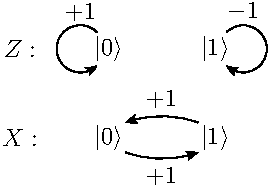
\includegraphics[]{pic-zx.pdf}
\end{center}
From this picture we can see that $Z$ acts by \emph{stabilizing} the
state $\ket{0}$ and anti-stabilizing the $\ket{1}$ state.
The $Z$ operator has been reduced 
to two operators each acting on a one dimensional subspace:
$Z = +1 \oplus -1.$
The $X$ operator serves to ``bitflip'' the state between
these two subspaces.

But what happens if we get confused and end up swapping
the $X$ and $Z$ operators? We would like to see the $X$ operator
as stabilizing / anti-stabilizing two subspaces, together with the
$Z$ operator as bitflipping between these.
The trick is to consider the \emph{orbits} of the operator
we hope to act as a stabilizer.
In this case there is only one orbit, $\ket{0}+\ket{1}$
and indeed, the $Z$ operator bitflips this to another state
$\ket{0}-\ket{1}$ that is anti-stabilized by $X.$

We are going to be considering Hamiltonians built from
summing operators of this form.
In this paper we use a ``neg-Hamiltonian'' convention,
to save complicating expressions with negative signs.
The ground space corresponds to the \emph{largest} eigenvalue.

So building a Hamiltonian from a single $X$ or $Z$ term,
we find the ground space as the stabilized space
by summing over the orbit of that term.
The other operator,
which we call the \emph{adjacent operator}, acts to bitflip
between the eigenspaces.

\underline{\bf Example 2.}
To further elucidate this idea we turn to another example,
which is a Hamiltonian built from three commuting and
independent operators:
$$
    \Ham = XXI + IXX + ZZZ.
$$
%We start with $\ket{000}$ and sum over the orbit of
%the terms in $\Ham.$ 
Starting with $\ket{000}$
the terms of the Hamiltonian generate an orbit
given by $$\mathrm{Orbit}(\ket{000}) = \{\ket{000}, \ket{011}, \ket{110}, \ket{101}\}.$$
Notice that the $ZZZ$ term fixes all these states.
Summing over this orbit we get the following ground state:
$$\mathrm{GS} = \ket{000}+\ket{011}+\ket{110}+\ket{101}.$$
%(Notice that the $ZZZ$ operator has no effect here.)
%\danbrowne{How do you compute this? ZZZ doesn't seem to play a role in generating this orbit. Why not?}

We select three adjacent operators
$ZII, IIZ,$ and $IXI,$
one for each of the stabilizer operators:
\begin{align*}
    ZII : \mbox{GS} &\mapsto \ket{000}+\ket{011}-\ket{110}-\ket{101} 
        \ \mbox{anti-stabilized by}\  XXI,\\
    IIZ : \mbox{GS} &\mapsto \ket{000}-\ket{011}+\ket{110}-\ket{101} 
        \ \mbox{anti-stabilized by}\  IXX,\\
    IXI : \mbox{GS} &\mapsto \ket{010}+\ket{001}+\ket{100}+\ket{111} 
        \ \mbox{anti-stabilized by}\  ZZZ.
\end{align*}

%For example, $ZII$ sends the ground state to
%$\ket{000}+\ket{011}-\ket{110}-\ket{101}$
%which is anti-stabilized by $XXI.$
These adjacent operators form an abelian group
%\danbrowne{It doesn't seem that it is necessary for this to be abelian via your definition. Are you demanding that it be abelian? If so, you should modify your definition. }
of order $2^3 = 8$ and by applying each element of
this group to the ground state we get a basis
of our state space, which we call a \emph{symmetry
invariant basis.}

The adjacent operators are not unique in general. 
For this example we could have also chosen $IZZ, ZZI, XXX.$

\underline{\bf Example 3.}
Now we consider a four qubit example:
$$
    \Ham = XXII + IIXX + ZIZI + IZIZ.
$$
This time the terms of the Hamiltonian do not generate 
an abelian group.
We will call this group, as generated by the terms in the Hamiltonian,
the \emph{gauge group}, $G$.
The \emph{stabilizer} subgroup of $G$ will be the elements of $G$
that commute with every other element in $G.$
By inspection we see this group is generated by $\Stab_0=\{XXXX, ZZZZ\}.$
%\danbrowne{What sets the phases of these operators? Are they arbitrarily chosen?}
We can extend these generators to a complete independent generating
set for $G$ using the operators  $R_0=\{XXII, ZIZI\}.$
These $R_0$ operators generate the \emph{reduced gauge group} $R.$
The operators adjacent to $\Stab_0$ we
call the \emph{error operators} $T_0$. 
We choose $T_0 = \{ZZZI, IIIX\}.$
(Once again, these are not unique.)
%\danbrowne{There's no unique choice here, so it's a bit misleading to call them "the adjacent operators". }
The \emph{logical operators} are the $n$-qubit 
Pauli operators outside of the group
$G$ that commute with $G.$
In this case they are generated by $L_0 = \{XIXI, ZZII\}.$
All of this can be summarized in a table of adjacent pairs:
\begin{center}
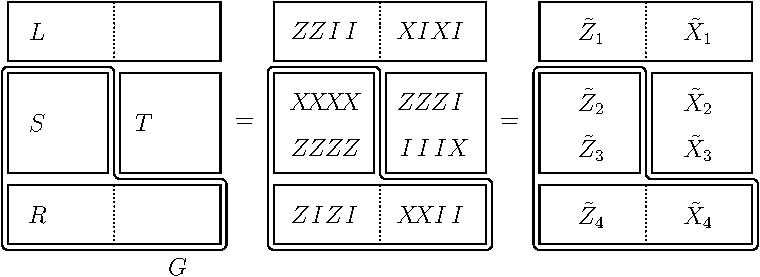
\includegraphics[]{pic-gauge4.pdf}
\end{center}
where the number of rows equals $n,$ 
each operator commutes with operators on other rows,
and anticommutes with the operator on the same row. 
There is no need to include any phases ($\pm I$) in these tables
because phases commute with everything.
If we take all the entries in the left column
we get the operators 
$\{ ZZII, XXXX, ZZZZ, ZIZI \}.$ 
These generate an abelian group 
that stabilizes the
state $\ket{\psi} = \ket{0000}+\ket{1111}.$
Let $r$ be the gauge operator $XXII$ adjacent to the 
stabilizer $ZIZI$,
The state $\ket{\psi}$ then lies in the $G-$orbit 
$$
\{\ket{\psi}, r\ket{\psi}\} = \{\ket{0000}+\ket{1111}, \ket{1100}+\ket{0011}\}.
$$
We use the $T_0$ operators $t_1=ZZZI$ and $t_2=IIIX$
to list three other $G-$orbits:
$$
\{t_1 \ket{\psi}, t_1 r\ket{\psi}\}, 
\{t_2 \ket{\psi}, t_2 r\ket{\psi}\}, 
\{t_1 t_2 \ket{\psi}, t_1 t_2 r\ket{\psi}\}.
$$
So now we have sixteen vectors, forming an orthogonal basis for the state space.
This is the symmetry invariant basis for this Hamiltonian.

We can now arrange these basis vectors on the vertices of a four dimensional hypercube,
such that each dimension corresponds to one of the adjacent $\tilde{X}_i$ bitflip
operators.
%drawn poorly with only two dimensions below.
Such an arrangement has a cartesian product
structure which induces a tensor product decomposition of
the original state space that corresponds to the $\tilde{X}_i:$
\begin{center}
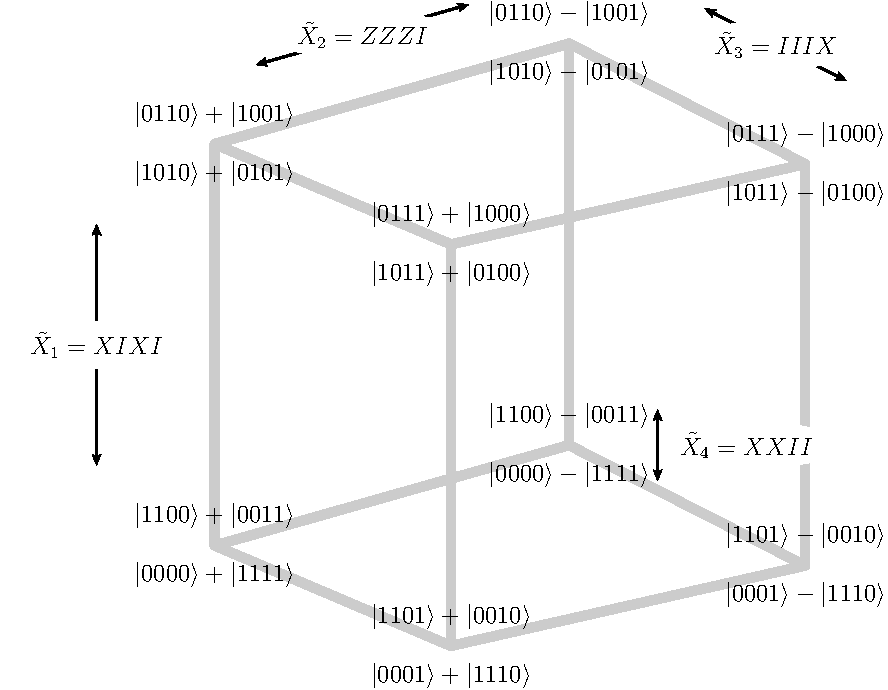
\includegraphics[width=0.7\columnwidth]{pic-operators.pdf}
\end{center}
The Hamiltonian acts on states by left multiplication.
Because this action
is a sum of gauge group elements,
it will decompose into blocks,
one for each $G-$orbit.
We depict this action as a weighted graph, where we omit edges
with zero weight:
\begin{center}
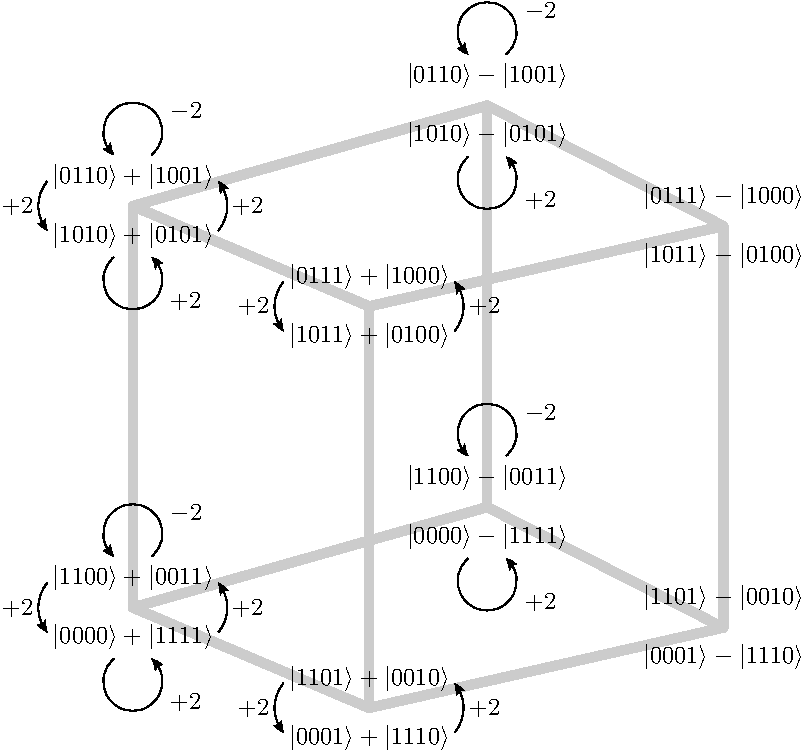
\includegraphics[width=0.7\columnwidth]{pic-orbit.pdf}
\end{center}

\def\Xt{\tilde{X}}
\def\Zt{\tilde{Z}}

Equivalently we use this basis to 
write the matrix for the Hamiltonian in
block diagonal form:
$$
\Ham = 
\left( \begin{array}{cccc}
2(X+Z) & 0 & 0 & 0 \\
0  & 2X & 0 & 0 \\
0  & 0 & 2Z & 0 \\
0  & 0 & 0 & 0 \\
\end{array} \right) \otimes I
$$
This block diagonal form will be worked out for
general gauge group $G$ below and summarized in Section 2.2.6.

%\todo{XXX and now for another formula}
%\begin{align*}
%\Ham &= XXII + IIXX + ZIZI + IZIZ \\
%  &= \Xt_4 + \Zt_2\Xt_4 + \Zt_4 + \Zt_3\Zt_4 \\
%  &= (I+\Zt_2)\Xt_4 + (I+\Zt_3) \Zt_4.
%\end{align*}

\section{Group representations}\label{GroupReps}

\subsection{The Pauli group}

The Pauli group $\Pauli_1$ is normally 
defined as a set of matrices closed under
matrix multiplication,\footnote{The original definition of the Pauli
group also includes an imaginary unit $i$, which we
do not include. So perhaps this should be called the
\emph{real} Pauli group.}
but we can define it abstractly
as the group generated
by the (abstract) elements $\{\omega, X, Z\}$ with
relations as follows:
$$
\omega^2=I,\ X^2=I,\ Z^2=I,\ \omega X\omega X=I,\ \omega Z\omega Z=I,\ \mbox{and}\  \omega ZXZX=I,
$$
where $I$ is the group identity.
Actually, $\omega $ is generated by $X$ and $Z$,
%\danbrowne{Perhaps mention that omega represents -1 here.  You should also mention that this is not the standard definition of the Pauli group, as you have neglected i.  In particular XY is not hermitian. Does it matter?}
so it is not necessary to include $\omega $ in the generating set,
but here it simplifies the relations.
%\footnote{We leave out $Y$ because...}
This group has eight elements, and is isomorphic to the dihedral group $D_4$,
the symmetry group of a square.

To define
the {\it $n$-qubit Pauli group} $\Pauli_n$, 
we use the $2n+1$ element 
generating set 
$$\{\omega , X_1, .., X_n, Z_1, .., Z_n\}$$
with relation $\omega^2=I$ as before, and
\begin{equation}\label{presentation}
\begin{array}{c}
X_i^2=I,\ Z_i^2=I,\ \omega X_i\omega X_i=I,\ \omega Z_i\omega Z_i=I,\ \omega Z_iX_iZ_iX_i=I, 
\mbox{\ for\ } i=1,...n,\\
X_iX_jX_iX_j=I,\ 
Z_iZ_jZ_iZ_j=I,\ 
Z_iX_jZ_iX_j=I, \mbox{\ for\ } i, j = 1,..,n,\ i\ne j.
\end{array}
\end{equation}

This abstract approach to the definition of a group is known as
a group \emph{presentation}. In general, this is a set of
generators together with a set of relations satisfied
by these generators.

Note that each of the generators squares to the identity,
and of these, only $\omega$ commutes with every element of $\Pauli_n.$
%Note that $\omega$ commutes with all elements of $\Pauli_n$
%and squares to the idenity, 
Therefore we will write $\omega$ as $-I,$
similarly $\pm I$ will denote the
set $\{\omega, I\},$ and $-X$ is $\omega X$, etc.

We write the group commutator as
$[[g, h]]:=ghg^{-1}h^{-1}$
and note the important commutation relation:
$$
    [[Z_i, X_j]] = 
    \left\{ \begin{array}{ll}
 -I &\mbox{if}\ i=j,\\
 I &\mbox{if}\ i\ne j.\end{array}\right.
$$
If we take an arbitrary $g\in \Pauli_n$
written as a product of the generators,
it follows that we can rewrite this
product uniquely as %in an ordered fashion:
$ g = \pm g_1 ... g_n $
where each $g_i$ is one of $I, Z_i, X_i$ or $X_i Z_i$
for $i=1,..,n.$
Therefore, the size of the
Pauli group is 
$$
    |\Pauli_n| = 2^{2n+1}.
$$

%Elements of $\Pauli_n$ that consist of
%products of only $I$ or $X$ will
%be call $X$-type elements (or operators)
%and similarly $Z$-type elements are 
%products of only $I$ or $Z$.
The subgroup of $\Pauli_n$ generated by
the elements $\{X_1,...,X_n\}$ % $\{X_i\}_{i=1,..,n}$ 
is denoted $\Pauli_n^X.$ These are the $X$-type
elements. Similarly,
 $\{Z_1,...,Z_n\}$ generates % $\{Z_i\}_{i=1,..,n}$ 
the subgroup of $Z$-type elements $\Pauli_n^Z$.

\subsection{Subgroups of the Pauli group}

We now define an {\it $n-$qubit gauge group} to be 
any non-abelian subgroup $G$ of $\Pauli_n,$
defined by a set of generators $G_0\subset \Pauli_n,$
%for some subgroup $G$ of $\Pauli_n:$
$$ G := \langle G_0\rangle.$$
%We will assume $G$ is not abelian, which 
%%is equivalent to the condition that $-I\in G.$ % No! {-I, I} is abelian...
%implies that $-I\in G.$
Because $G$ is not abelian, it follows that $-I\in G.$
We also restrict $G_0$ to only contain Hermitian operators,
which is equivalent to requiring that $g^2=I$ for all $g\in G_0.$

Now let $\Stab$ be the largest subgroup of $G$ not containing
$-I.$
$\Stab$ is then an abelian subgroup,
also known as the {\it stabilizer} subgroup.
%(Note that each of the stabilizers commutes with the Hamiltonian.)
$G$ decomposes as a direct product:
$$G = \Stab\times R,$$
where $R\cong \Pauli_r$ for some $1\le r\le n,$
and $\Stab\cong \Z_2^{m}$ for $0\le m<n.$
Therefore, 
$$|G| = |\Stab| |R| = 2^{m+2r+1}.$$
We call $R$ the {\it reduced gauge group}.
We consider both $\Stab$ and $R$ to be subgroups of $G.$
%Let $\phi:\Pauli_r\to R$ be a group isomorphism,
Let $\phi:R\to \Pauli_r$ be a group isomorphism,
%then $R_0 := \{\phi(X_i), \phi(Z_i)\}_{1\le i\le r}$
%then $R_0 := \{\phi(X_i), \phi(Z_i)\}_{i=1,..,r}$
then $R_0 := \{\phi^{-1}(X_i), \phi^{-1}(Z_i)\}_{i=1,..,r}$
is a set of independent generators of $R.$
We also let $\Stab_0$ be a set of $m$ independent generators of $\Stab.$

To find the cosets of $G$ in $\Pauli_n$ we take
the group closure of $\Pauli_n-G$; when this is non-empty
we only need to add $I$ and $-I.$
This is another
gauge group, whose reduced gauge group is known as
the {\it logical} operators $L$, and whose 
stabilizer subgroup is known as the {\it error} operators $T.$
Now any coset of $G$ can be written as $ltG$ with
$l\in L$ and $t\in T.$
The size of $T$ equals the size of $\Stab$: $|T|=|\Stab|=2^m.$
If we let $L_0$ be an independent generating set for $L$
then we have the important formula:
\begin{align}
n &= \frac{1}{2}|L_0| + |\Stab_0| + \frac{1}{2}|R_0|\\
  &= k + m + r
\end{align}
We summarize the information in this section in a table
of Pauli group elements arranged in
two columns and $n$ rows:
\begin{center}
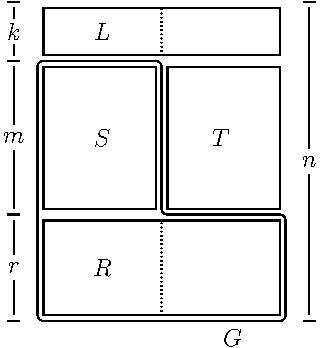
\includegraphics[]{pic-canonical.pdf}
\end{center}
Here we show the $2n$ generators of $\Pauli_n$ arranged 
so that each row contains a pair of generators,
where each such generator anti-commutes with the operator on the same row and
commutes with all the other operators in the table.
Note that this is exactly the definition of the Pauli group
via a presentation given in the previous section.
Furthermore, the table shows $2k$ generators
of $L$, $m$ generators each for $S$ and $T,$ and $2r$
generators of $R.$
The gauge group $G$ encloses $R$ and $S$, and one can
immediately see how $L$ and $T$ also form a gauge group.


\subsection{Representations of the Pauli group}

We now define the
{\it Pauli representation} 
of the Pauli group as a group homomorphism:
$$
    \rho_{\mathrm{pauli}} : \Pauli_n \to \GL(\Complex[2^n])
$$
where $\Complex[2^n]$ is the $2^n$-dimensional state space of $n$ qubits.
On the independent generators 
$\{X_1, .., X_n, Z_1, .., Z_n\},\ \rho_{\mathrm{pauli}}$
is defined as the following tensor product of $2\times 2$ matrices:

%$$
%\rho_{\mathrm{pauli}}(X_i) := \bigotimes_{j=1}^n \left\{ \begin{array}{ll}
%\left( \begin{array}{ll}
%1&0\\
%0&1\end{array} \right) &\mbox{for $j\ne i$,}\\
%\\
%\left( \begin{array}{ll}
%0&1\\
%1&0\end{array} \right) &\mbox{for $j=i$} \end{array}
%\right\},\ 
%\rho_{\mathrm{pauli}}(Z_i) := \bigotimes_{j=1}^n \left\{ \begin{array}{ll}
%\left( \begin{array}{ll}
%1&0\\
%0&1\end{array} \right) &\mbox{for $j\ne i$,}\\
%\\
%\left( \begin{array}{rr}
%1&0\\
%0&-1\end{array} \right) &\mbox{for $j=i$}\end{array}
%\right\}.
%$$

\begin{align*}
\rho_{\mathrm{pauli}}(X_i) := &\bigotimes_{j=1}^n \left\{ \begin{array}{ll}
\left( \begin{array}{ll}
0&1\\
1&0\end{array} \right) &\mbox{for $j=i$}\\
\\
\left( \begin{array}{ll}
1&0\\
0&1\end{array} \right) &\mbox{for $j\ne i$} \end{array}
\right.\\
\rho_{\mathrm{pauli}}(Z_i) := &\bigotimes_{j=1}^n \left\{ \begin{array}{ll}
\left( \begin{array}{ll}
1&0\\
0&-1\end{array} \right) &\mbox{for $j=i$}\\
\\
\left( \begin{array}{rr}
1&0\\
0&1\end{array} \right) &\mbox{for $j\ne i$}\end{array}
\right.
\end{align*}

%on $n$ qubits, $\Pauli_n,$
%as the set of $n$-fold tensor products
%of the matrices $\pm I, X, Z:$
%$$
%I = \left( \begin{array}{ll}
%1&0\\
%0&1\end{array} \right),\quad
%X = \left( \begin{array}{ll}
%0&1\\
%1&0\end{array} \right),\quad
%Z = \left( \begin{array}{ll}
%1&0\\
%0&-1\end{array} \right).
%$$

Normally the image of 
$\rho_{\mathrm{pauli}}$ is thought of as the
Pauli group itself, and we are indeed free to think
that way because $\rho_{\mathrm{pauli}}$ is a group
isomorphism.

Given a group representation $\rho:G\to GL(V)$
the {\it character} of $\rho$ is a function
$\chi_\rho:G\to \Complex$ given by
$$
    \chi_\rho(g) = \mbox{Tr}\ \rho(g).
$$

Given two functions $u,v : G \to \Complex$ 
we define the following inner product:
$$
    \langle u, v \rangle := \frac{1}{|G|} \sum_{g\in G} u(g) \overline{v(g)}.
$$

The character of the Pauli representation, $\chi_{{pauli}}:\Pauli_n\to\Complex$
is given by:
$$
\chi_{{pauli}}(g) = \sum_{v \in basis} \langle v | \rho_{{pauli}}(g) | v \rangle
    = \left\{ \begin{array}{ll}
 \pm 2^n &\mbox{if}\ g=\pm I\\
 0 &\mbox{otherwise}\end{array}\right.
$$

Since $|\Pauli_n|=2^{2n+1}$ it follows that
$\langle\chi_{pauli},\chi_{pauli}\rangle = 1$ and
so $\rho_{pauli}$ is an irreducible representation of $\Pauli_n.$

%It turns out %(see Appendix for details)
%that $\rho_{\mathrm{pauli}}$ is an
%irreducible representation ({\it irrep}) of $\Pauli_n$. 
The only other irreps of $\Pauli_n$ are 
the $1$-dimensional irreps $\rho:\Pauli_n\to\Complex$
defined on the independent generators as:
    $$ \rho(X_i) = \pm 1,\quad \rho(Z_i) = \pm 1.$$

So we have $2^{2n}$ many $1$-dimensional irreps,
and a single $2^n$-dimensional irrep.
Summing the squares of the dimensions
shows that we have a complete set of irreps of $\Pauli_n.$

%\subsection{Representations of stabilizer groups}
%
%Any abelian subgroup $\Stab\subset \Pauli_n$
%that does not contain $-I$ we call a stabilizer group.
%The reason for this name is...


\subsection{Representations of gauge groups}

%Our next job will be to find the irreps of {\it subgroups} of $\Pauli_n.$
Although $\rho_{\mathrm{pauli}}$
restricted to a gauge group $G\subset\Pauli_n$ serves as a representation
of $G$ it is no longer irreducible.
Our aim will be to decompose $\rho_{\mathrm{pauli}}$ into irreps of $G.$

The $1$-dimensional irreps $\rho:G\to \Complex,$
are now defined by
specifying the action of $\rho$ on the independent generators:
$$
    \rho(h)=\pm 1\ \mbox{for}\ h\in \Stab_0,
    \quad \rho(\phi^{-1}(X_i)) = \pm 1,\quad \rho(\phi^{-1}(Z_i)) = \pm 1.
$$
This gives all $2^{m+2r}$ of the $1$-dimensional irreps.
%These will turn out not to be used below.

The $2^r$-dimensional irreps are given by:
$$
    \rho(h) = \pm I^{\otimes r}\ \mbox{for}\ h\in \Stab_0,
    \quad \rho(\phi^{-1}(X_i)) = X_i,\quad \rho(\phi^{-1}(Z_i)) = Z_i.
$$
We are free to choose the signs of the $\rho(h)$ for each $h\in \Stab_0.$
Hence there are $2^m$ many of these irreps.
Each such choice corresponds to the choice of a {\it syndrome} vector $s(h)=\pm 1$, for $h \in \Stab_0,$
or alternatively, choice of an element $t\in T:$
$$
    \rho^1_t(h) = \left\{ \begin{array}{ll}
 I^{\otimes r}\ &\mbox{if $th=ht$}\\
 -I^{\otimes r}\ &\mbox{if $th=-ht$}\end{array} \right. %\right\}\mbox{for}\ h\in \Stab_0.
$$

%Finally, there are $2^m$ many $2^r$-dimensional irreps $\rho_t$
%which are labeled by $t\in T$ and defined as
%$$
%    %\rho_t(h)=\pm I^{\otimes 2^r}\ \mbox{for}\ h\in \Stab_0,
%    %\rho_t(h)= [t,h] = th^{-1}th^{-1} = \pm I^{\otimes 2^r}\ \mbox{for}\ h\in \Stab_0,
%    \rho_t(h) = \left\{ \begin{array}{ll}
% I^{\otimes 2^r}\ &\mbox{if $th=ht$}\\
% -I^{\otimes 2^r}\ &\mbox{if $th=-ht$}\end{array} \right\}\mbox{for}\ h\in \Stab_0,
%    \quad \rho_t(\phi^{-1}(X_i)) = X_i,\quad \rho_t(\phi^{-1}(Z_i)) = Z_i.
%$$

%For $G$ a subgroup of $\Pauli_n$, and decomposition
Because $G$ decomposes 
into a direct product $G=\Stab\times \Pauli_r$ we have the
following representations:
$$
    \rho_t(g) = \rho^1_t(h) \rho^r_{pauli}(g'),
$$
where $g=hg'$, $h\in \Stab$, $g'\in \Pauli_r$ 
%and $\rho_1(h)$ is a $1$-dimensional representation of $\Stab$.
and $\rho^r_{pauli}$ is the $r$-qubit Pauli representation.
The character for this representation is:
$$
\chi_{t}(hg') = \rho_t^1(h) \sum_{v \in basis} \langle v | \rho^r_{{pauli}}(g') | v \rangle
    = \left\{ \begin{array}{ll}
 \pm 2^r\rho_t^1(h) &\mbox{if}\ g'=\pm I\\
 0 &\mbox{otherwise}\end{array}\right.
$$

We have that $|G|=2^{2r+m+1}$ and so
$\langle\chi_{t},\chi_{t}\rangle = 1$ and
$\rho_t$ is an irreducible representation of $G.$
We now count the occurrences of 
this representation in $\rho^r_{pauli}$:
\begin{align*}
\langle\chi^r_{pauli},\chi_{t}\rangle &= \frac{1}{|G|}\sum_{g\in G} \chi^r_{pauli}(g)\overline{\chi_{t}(g)} \\
&= \frac{1}{2^{2r+m+1}} \sum_{g=\pm I} 2^n 2^r = \frac{2^{n+1+r}}{2^{2r+m+1}} = 2^k
\end{align*}
where $k$ is the number of logical qubits so that $n=r+m+k.$

%\noindent{\bf Theorem.}
%Using characters one can show that
%on a subgroup $G$ of $\Pauli_n$ the
In summary, the Pauli representation decomposes into 
$2^m$ many irreps $\rho_t,$ 
each with dimension $2^r,$ 
and appearing with multiplicity $2^k:$
$$
    \rho_{\mathrm{pauli}} = 
        \bigoplus_{t\in T}\ \rho_t \otimes I^{\otimes k}
$$
%where we label the $2^r$-dimensional irreps by $t\in T.$
%See appendix for details.

\subsection{Symmetry invariant basis}

In general, given a representation $\rho:G\to \GL(V)$
and the character of some irreducible representation $\chi:G\to \C$
the following operator 
$P:V\to V$
projects onto the subspace on which
this irreducible representation acts:
$$
    P := \frac{d}{|G|} \sum_{g\in G} {\overline{\chi(g)}} \rho(g).
$$
where $d$ is the dimension of the irreducible representation.
We can use this to calculate projectors onto the irreps $\rho_t$ in $\rho_{pauli}$:
\begin{align*}
P_t &= \frac{d}{|G|} \sum_{g\in G} \overline{\chi_t(g)} \rho_{pauli}(g) \\
    &= \frac{d}{|G|} \sum_{h\in \Stab}\sum_{g\in R} \overline{\chi_t(hg)} \rho_{pauli}(hg) \\
    &= \frac{d}{|G|} 2^{2r} \sum_{h\in \Stab} {\rho^1_t(h)} \rho_{pauli}(h) \\
    &= \frac{1}{2^m} \sum_{h\in \Stab} {\rho^1_t(h)} \rho_{pauli}(h).
\end{align*}

We can also write this as a product of projectors onto
the $\pm 1$ eigenspaces of stabilizers $\rho_{pauli}(h)$ for $h\in \Stab.$
Choose generators $h_1,...,h_m$ of $S$
and then the projectors onto the $\pm 1$ eigenspace of $\rho_{pauli}(h_i)$ are
$$
P^i_t = \frac{1}{2} \bigl(I^{\otimes n} \pm \rho_{pauli}(h_i) \bigr)
$$
and we see that 
$$
P_t = \prod_{i=1,...,m} P^i_t 
    = \frac{1}{2^m} \bigl(I^{\otimes n} \pm \rho_{pauli}(h_1)\bigr)
    ...\bigl(I^{\otimes n} \pm \rho_{pauli}(h_m)\bigr).
$$
This projector will have rank $2^{k+r}$ and
$$
U := \sum_{t\in T} P_t
$$
is a unitary transformation that sends
physical qubits to encoded qubits.


\subsection{The Hamiltonian}

The Hamiltonian of interest is 
an operator $\Ham:\Complex[2^n]\to\Complex[2^n]$:
%and normally defined
%as the negative sum of terms from $G_0,$ but here
%we will reverse the sign:
$$ \Ham := \sum_{g\in G_0} \rho_{\mathrm{pauli}}(g).$$
Using the above decomposition we find:
\begin{align*}
    \Ham &= \sum_{g\in G_0}\ \bigoplus_{l\in L, t\in T}\ \rho_t(g)\\
         &= \bigoplus_{l\in L, t\in T} \sum_{g\in G_0}\ \rho_t(g).
\end{align*}
%The goal is to decompose $\Ham$ into blocks as
%$$
%    \Ham = \bigoplus_{\mathrm{irrep}\rho} \sum_{g\in G_0}\ \rho(g),
%$$
We will notate each block as
$\Ham_t := \sum_{g\in G_0}\rho_t(g)$
for each irrep $\rho_t$ appearing in $\Ham.$
\begin{framed}
\noindent{\bf Fact 0:}
The Hamiltonian is block diagonalized, with blocks indexed by operators $t$ in
the abelian group $T$ and multiplicity $2^k:$
$$
    \Ham =  \bigoplus_{t\in T}\ \Ham_t \otimes I^{\otimes k}.
$$
\end{framed}
%Writing $I$ for the identity element of $T$ we write the corresponding
%block of the Hamiltonian as $\Ham_{0,0}.$

More generally, we can assign real valued weights
$J_g\in\R$
to each operator $g\in G_0,$
\begin{align*}
    \Ham = \sum_{g\in G_0} J_g \rho_{\mathrm{pauli}}(g)
            = \bigoplus_{l\in L, t\in T} \sum_{g\in G_0}\ J_g \rho_t(g).
\end{align*}
In other words, using weights does not change the block structure of $\Ham.$

In the following sections we will forget the distinction 
between $g$ and $\rho_{\mathrm{pauli}}(g)$,
so terms such as $Z$ and $X$ can be understood
as the corresponding Pauli linear operators.

%%%%%%%%%%%%%%%%%%%%%%%%%%%%%%%%%%%%%%%%%%%%%%%%%%%%%%%%%%%%%%%%%%%%%%%%%%%%%%%
%
%%%%%%%%%%%%%%%%%%%%%%%%%%%%%%%%%%%%%%%%%%%%%%%%%%%%%%%%%%%%%%%%%%%%%%%%%%%%%%%
%

\section{Applications}

We now use the tools built so far
to analyze two examples of gauge code Hamiltonians.
The above procedure is not entirely automatic,
it relies on extracting the isomorphism $\phi$,
but when this can be made to work it works surprisingly well.

%%%%%%%%%%%%%%%%%%%%%%%%%%%%%%%%%%%%%%%%%%%%%%%%%%%%%%%%%%%%%%%%%%%%%%%%%%%%%%%
%
%%%%%%%%%%%%%%%%%%%%%%%%%%%%%%%%%%%%%%%%%%%%%%%%%%%%%%%%%%%%%%%%%%%%%%%%%%%%%%%
%

\subsection{The 2D compass model}

Here we consider the two-dimensional compass model \cite{Bacon2006}.
We coordinatize the qubits on a square 
lattice of\ $l\times l$\ sites,
$(i, j)$\ for\ $1\le i, j\le l.$
This gives $n = l^2.$
For the single qubit Pauli operators acting on site
$(i, j)$ we coordinatize with subscripts $ij$, 
with $i$ and $j$ understood modulo $l$.
The generators of the gauge group are
$$
    G_0 = \big\{ X_{ij}X_{i,j+1},\ Z_{ij}Z_{i+1,j}\ \mbox{for}\ 1\le i, j\le l\big\}.
$$
We write generators of the reduced
gauge group in anti-commuting pairs:
$$
    R_0 = \big\{ X_{i1}X_{ij},\ Z_{1j}Z_{ij}\ \mbox{for}\ 2\le i, j\le l\big\}.
$$
This makes it clear the isomorphism $\phi : R \to \Pauli_r$ to use,
and we again use pairs $i,j$ to coordinatize $\Pauli_r$:
$$
    \phi(X_{i1}X_{ij}) = X_{i-1,j-1}, \ \ \phi(Z_{1j}Z_{ij}) = Z_{i-1,j-1},\ \mbox{for}\ 2\le i, j\le l.
$$
The generators for the stabilizers are
$$
    \Stab_0 = \big\{ \prod_{i=1}^l X_{ij}X_{i,j+1},\ \prod_{i=1}^l Z_{ji}Z_{j+1,i}\ \mbox{for}\ 1\le j\le l-1\big\}.
$$
The logical operators are generated by $L_0 = \big\{ \prod_i X_{i1}, \prod_j Z_{1j} \}.$
These sets have cardinalities:
$$|G_0|=2l^2,\ |R_0| = 2(l-1)^2,\ |\Stab_0| = 2(l-1).$$
%And we note that $\frac{1}{2}|L_0| + |\Stab_0| + \frac{1}{2}|R_0| = n.$
And we note that $k+m+r=n$ is satisfied.
%Now we can define the irreps of $G$.
Now we write down the values of the
irreps on the gauge operators.
Here we define each irrep using a pair 
of syndrome vectors $s_X$ and $s_Z:$
\begin{align*}
\rho(X_{i1} X_{i2}) &= X_{i-1,1} &
%\rho(Z_{1i} Z_{2i}) &= Z_{1,i-1} &\mbox{for}\ 2\le i\le l\\
\rho(Z_{1i} Z_{2i}) &= Z_{1,i-1} \\&&&\mbox{for}\ 2\le i\le l\\
\rho(X_{il} X_{i1}) &= X_{i-1,l-1} &
%\rho(Z_{li} Z_{1i}) &= Z_{l-1,i-1} &\mbox{for}\ 2\le i\le l\\
\rho(Z_{li} Z_{1i}) &= Z_{l-1,i-1} \\&&&\mbox{for}\ 2\le i\le l\\
\rho(X_{ij} X_{i,j+1}) &= X_{i-1,j-1} X_{i-1,j} &
%\rho(Z_{ji} Z_{j,i+1}) &= Z_{j-1,i-1}Z_{j,i-1} &\mbox{for}\ 2\le i\le l, 2\le j<l\\
\rho(Z_{ji} Z_{j,i+1}) &= Z_{j-1,i-1}Z_{j,i-1} \\&&&\mbox{for}\ 2\le i\le l, 2\le j<l\\
\rho(X_{1j} X_{1,j+1}) &= s_X(j-1) \prod_{i=1}^{l-1} X_{i,j-1} X_{ij} &
%\rho(Z_{j1} Z_{j+1,1}) &= s_Z(j-1) \prod_{i=1}^{l-1} Z_{j-1,i} Z_{ji} &\mbox{for}\ 2\le j<l\\
\rho(Z_{j1} Z_{j+1,1}) &= s_Z(j-1) \prod_{i=1}^{l-1} Z_{j-1,i} Z_{ji} \\&&&\mbox{for}\ 2\le j<l\\
\rho(X_{11} X_{12}) &= \prod_{j=1}^{l-1}s_X(j) \prod_{i=1}^{l-1} X_{i1} &
\rho(Z_{11} Z_{21}) &= \prod_{j=1}^{l-1}s_Z(j) \prod_{i=1}^{l-1} Z_{1i}.
\end{align*}
Note the transposition symmetry between the $X$ and $Z$-type operators.
We sum all these terms to find 
the form of the Hamiltonian in each block:
$$
\Ham_\rho = \sum_{g\in G_0} \rho(g) = \sum_{1\le i,j<l} \rho(X_{ij}X_{i,j+1}) + \rho(Z_{ij}Z_{i+1,j}).
$$
We note that in \cite{Brzezicki2013},
they perform a
spin transformation of the compass model
which also results in an $(l-1)\times(l-1)$ lattice
of spins and identical Hamiltonian up to some signs.

%Note that the form of each of the Hamiltonian blocks $H_t$
%comes from another gauge code.
%In this case it has some non-local operators, as well as $\pm 1$ factors
%which can be subsumed into the gauge code as operators $\pm I.$

%We have the following important fact which we will prove in section \ref{spectra} below:
%\begin{framed}
%\noindent{\bf Fact 1:}
%The blocks $H_t$ of a CSS gauge code Hamiltonian are also CSS.
%\end{framed}
%
%By counting dimensions we can conclude the following:
%\begin{framed}
%\noindent{\bf Fact 2:}
%Each block $H_t$ has non-degenerate groundspace.
%\end{framed}
%
%\emph{!! check what happens with weights $\pm 1.$}

%\fbox{\parbox[b]{5cm}{This is long text that will be wrapped once it reaches five centimeters.}}

%%%%%%%%%%%%%%%%%%%%%%%%%%%%%%%%%%%%%%%%%%%%%%%%%%%%%%%%%%%%%%%%%%%%%%%%%%%%%%%
%

%\subsection{The 1D models}
%
%We define the \emph{Jordan-Wigner presentation} of $\Pauli_n$
%using the following set of $2n$ independent generators \cite{Jordan1928}:
%$$
%%\mathrm{JW}_Z :=
%\big\{c_{2j}^Z:=Z_1...Z_{j-1} X_j,\ c_{2j+1}^Z:=Z_1...Z_{j-1} Y_j\ \ 
%\mbox{for}\ 1\le j\le n\big\}.
%$$
%That these operators are independant and
%generate $\Pauli_n$ can be seen by considering
%the abelianization of $\Pauli_n$ which is the group $\Z_2^{2n}.$
%There are two other ways of writing this presentation:
%\begin{align*}
%%\mathrm{JW}_X &:=
%\big\{c_{2j}^X:=X_1...X_{j-1} Y_j,\ c_{2j+1}^X:=X_1...X_{j-1} Z_j\ \ 
%\mbox{for}\ 1\le j\le n\big\},\\
%%\mathrm{JW}_Y &:=
%\big\{c_{2j}^Y:=Y_1...Y_{j-1} X_j,\ c_{2j+1}^Y:=Y_1...X_{j-1} Z_j\ \ 
%\mbox{for}\ 1\le j\le n\big\}.
%\end{align*}
%
%%This example shares features of both the previous and the next examples.
%The $XY$-model 
%lives on a one dimensional chain of $n$ qubits.
%We write the gauge group generators as
%$$
%    G_0 = \{ X_i X_{i+1}, Z_i Z_{i+1}\ \ \mbox{for}\ \ i=1,...,n \}
%$$
%with periodic boundary conditions.
%For $n$ even this model has no logical operators, one 
%$X$-type stabilizer and one $Z$-type stabilizer.
%With $n$ odd, there are no stabilizers and $k=1.$
%Normally the gauge operators are written as 
%$\{ X_i X_{i+1}, Y_i Y_{i+1} \ \mbox{for}\ i=1,...,n \}$
%but note that there is an automorphism of the Pauli group
%that sends $G_0$ to these operators.
%For $n$ even, this model is exactly solvable,
%and the gap goes to zero
%as the system size grows \cite{Lieb1961}.
%
%For the one dimensional transverse field
%Ising model, we have 
%$$
%    G_0 = \{ X_i, Z_i Z_{i+1}\ \ \mbox{for}\ \ i=1,...,n \},
%$$
%with periodic boundary conditions.
%This model has one 
%$X$-type stabilizer and no logical operators.
%This model is also exactly solvable, with gap going to zero
%as the system size grows \cite{Pfeuty1970}.


%http://arxiv.org/pdf/1504.01444 page 86.


%%%%%%%%%%%%%%%%%%%%%%%%%%%%%%%%%%%%%%%%%%%%%%%%%%%%%%%%%%%%%%%%%%%%%%%%%%%%%%%
%

\subsection{The Kitaev honeycomb model}


%\begin{figure*}[th!]
%\begin{center}
%        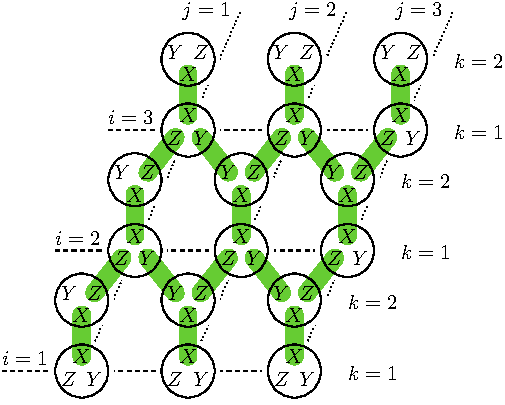
\includegraphics[width=0.6\columnwidth]{fig_00.pdf}
%\caption{
%Gauge generators have support on the edges of the honeycomb lattice.
%Qubits here are depicted as circles.
%}
%\label{honeycomb}
%\end{center}
%\end{figure*}


The Kitaev honeycomb model \cite{Kitaev2006} is built from spins on
the sites of a hexagonal lattice. 
The lattice of linear size $l$ has $n=2l^2$ sites
which we coordinatize using integer triples $i, j, k$
with $1\le j, k\le l$ and $k=1, 2.$
We use periodic boundary conditions so $i, j$ are
to be taken modulo $l$.
Gauge generators have support on the edges of the honeycomb lattice,
and we depict qubits here as circles:
\begin{center}
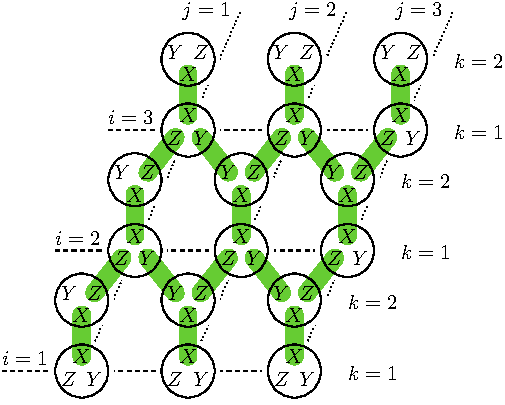
\includegraphics[width=0.6\columnwidth]{fig_00.pdf}
\end{center}
%See figure \ref{honeycomb}.
The edges of the lattice are in one-to-one
correspondence with the generators $G_0$:
$$
G_0 := \big\{X_{ij1}X_{ij2},\ Z_{ij2}Z_{i+1,j1},\ Y_{ij1}Y_{i-1,j+1,2}
\ \mbox{for}\ 1\le i,j\le l\big\}.
$$
Note that we make the definition $Y:=XZ$ for each site.\footnote{
This operator $Y$ is not Hermitian, but it only appears in a tensor pair in
the Hamiltonian and so these terms will be Hermitian.}
%\danbrowne{Can you do this? Please justify it? (Presumably ok since Y only occurs as a tensor pair). } 
Stabilizers are generated from closed strings of
gauge operators. 
For example, each hexagon gives a stabilizer
\begin{align*}
h_{ij}:&= 
X_{ij1}X_{ij2}
Z_{ij2}Z_{i+1,j1}
Y_{i+1,j1}Y_{i,j+1,2}
X_{i,j+1,2}X_{i,j+1,1}
Z_{i,j+1,1}Z_{i-1,j+1,2}
Y_{i-1,j+1,2}Y_{ij1}
\\
&= 
Z_{ij1} Y_{ij2} X_{i+1,j1}
Z_{i,j+1,2} Y_{i,j+1,1} X_{i-1,j+1,2}.
\end{align*}

And the two homologically non-trivial loops
give stabilizers:
$$
h_v := \prod_{i=1}^l Y_{i11} Y_{i12},\ \ 
h_h := \prod_{j=1}^l X_{1j2} X_{2j1}.
$$

This gives independent stabilizer generators $\Stab_0$
from each hexagon, less one, as well as $h_v$ and $h_h.$
%two homologically non-trivial loops.
The number of hexagons is $\frac{1}{2}n$ and
so we find $|\Stab_0|=\half n+1.$
There are no logical operators, so we
must have $|R_0|=n-2.$

%\begin{figure*}[th!]
%\begin{center}
%        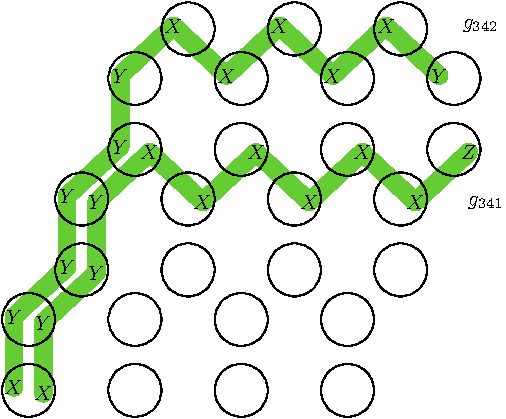
\includegraphics[width=0.5\columnwidth]{fig_01.pdf}
%%\caption{Two elements $g_{341}$ and $g_{342}$ of the set $R_0$}
%\caption{Two elements of the set $R_0$ corresponding
%to $i=3$, $j=4$ and $k=1,2.$}
%\label{jaws}
%\end{center}
%\end{figure*}

Now we construct a set of string operators $R_0$,
one for each site on the lattice, except for
the two sites $(1,1,1)$ and $(1,1,2).$
Each string $g_{ijk}\in R_0$
is constructed as the product of
gauge operators along a path starting at
$(1,1,1)$ and terminating at $(i,j,k).$
%See figure \ref{jaws}.

Two elements of the set $R_0$ corresponding
to $i=3$, $j=4$ and $k=1,2.$
\begin{center}
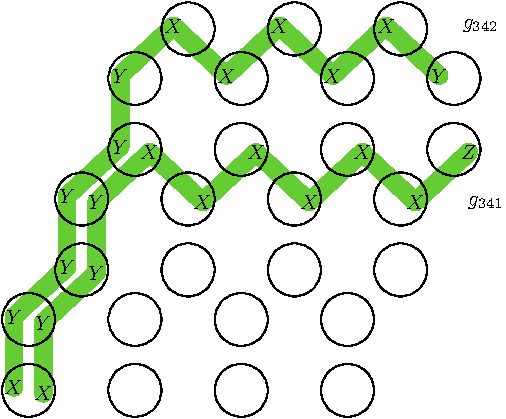
\includegraphics[width=0.5\columnwidth]{fig_01.pdf}
\end{center}

Each such path is built from two ``straight''
path segments, first in the $i$ direction
and then in the $j$ direction. 
The paths for operators $g_{ij1}$ and
$g_{ij2}$ coincide along the $i$ direction
but become disjoint in the $j$ direction:
the $g_{ij1}$ path goes around the bottom
of the hexagons and the $g_{ij2}$ path
goes around the top.
With periodic boundary conditions $R_0$ forms an
independent generating set of $R$ of size $n-2.$

We construct an isomorphism $\phi: R\to \Pauli_r$
by sending elements of $R_0$ bijectively
to the following independent generating
set of $\Pauli_r$:
$$
\big\{c_{2j}:=Z_1...Z_{j-1} X_j,\ c_{2j+1}:=Z_1...Z_{j-1} Y_j\ \ \mbox{for}\ 1\le j\le r\big\}.
$$
The bijection is constrained 
by setting $\phi(g_{ij1}):=c_{2j'+1}$
and $\phi(g_{ij2}):=c_{2j'}$
where $j'$ is chosen uniquely for each $i, j.$
The $c_j$ are paired Majorana fermion operators  \cite{Jordan1928, Kitaev2006}.

%We construct an isomorphism $\phi: R\to \Pauli_r$
%by setting $\phi(g_{ij1}):=c_{2j'}$
%and $\phi(g_{ij2}):=c_{2j'+1}$
%%we map 
%%elements of $R_0$ to the following independent generating
%where the $c_j$ form the following independent generating
%set of $\Pauli_r$:
%$$
%%\big\{\prod_{i=1}^{j-1} Z_i X_j,\ \prod_{i=1}^{j-1} Z_i Y_j\ \mbox{for}\ 1\le j\le r\big\}.
%\big\{c_{2j}:=Z_1...Z_{j-1} X_j,\ c_{2j+1}:=Z_1...Z_{j-1} Y_j\ \ \mbox{for}\ 1\le j\le r\big\}.
%$$

We check this is a group homomorphism by showing that relations
satisfied by elements of $R_0$ are satisfied by
their images under $\phi.$
All such relations are either of the form
$g^2=~\pm~I$, $gg'=\pm~g'g$, or
products thereof.
So it is sufficient to check squares of
elements and commutation relations.
Every element of $R_0$ anticommutes with
every other element of $R_0$, and this is true also
of the $c_j.$
Also, $g_{ij1}^2=-I$ and $g_{ij2}^2=I$ 
is preserved by $\phi$ because $c_{2j}^2=I$ and $c_{2j+1}^2=-I$.
Finally, $\phi$ is an isomorphism
because it is a bijection of two independent
generating sets.

The next step is to write each element of $G_0$
as a product of reduced gauge operators and stabilizers.
The key thing to note is that the product of two
operators $g_{ijk}, g_{i'j'k'}\in R_0$ gives a string
operator between the sites $(i,j,k)$ and $(i',j',k')$.
And {\it any} string operator between these
two sites can then be generated by using stabilizers to
``deform'' the string $g_{ijk}g_{i'j'k'}.$
For example, taking the product
of two operators from $R_0$ that differ
by one path segment gives the following:
\begin{align*}
Z_{ij2}Z_{i+1,j,1} &= g_{ij2} g_{i+1,j,1} \\
%&\mbox{for}\ \  1\le i<l,\ 1\le j\le l, \ \ \mbox{except}\ \  (i,j)=(1,1) \ \ \mbox{or}\ \ (l,1)\\
Y_{i+1,j,1}Y_{i,j+1,2} &= g_{i+1,j,1}g_{i,j+1,2}
%&\mbox{for}\ \  1\le i,j\le l, \ \ \mbox{except}\ \  (i,j)=(1,1) \ \ \mbox{or}\ \ (l,1).
\end{align*}
We need the homologically non-trivial stabilizers to get these:
\begin{align*}
Z_{lj2}Z_{1j1} &= h_v g_{lj2} g_{1j1} &\mbox{for}\ \  2\le j\le l
\end{align*}
And the $X_{ij1}X_{ij2}$
gauge operators can be generated
by the product of 
$g_{ij1}g_{ij2}$ and the enclosed hexagon stabilizers:
$$X_{ij1}X_{ij2}=g_{ij1}g_{ij2}\prod_{j'=1}^{j-1} h_{ij'}.$$

The only $G_0$ operators that are not 
quadratic in $R_0$ operators are the five
operators that touch either of the sites
$(1,1,1)$ or $(1,1,2)$.

So each block in the Hamiltonian
is seen to be quadratic in the $c_j$ plus
five other Pauli operator terms which we denote as $\Lambda_\rho$:
$$
    \Ham_\rho = \sum_{ij} \Gamma_{ij}(\rho) c_i c_j + \Lambda_\rho
$$
The coefficients $\Gamma_{ij}$ are dependant on the irrep $\rho.$

In \cite{Kells2009} they introduce a similar set of
mutually anti-commuting string operators $R_0.$

%%%%%%%%%%%%%%%%%%%%%%%%%%%%%%%%%%%%%%%%%%%%%%%%%%%%%%%%%%%%%%%%%%%%%%%%%%%%%%%
%

\def\Cn{\Complex[2^n]}
\def\Cr{\Complex[2^r]}
%\def\Field{\mathcal{F}_2}
%\def\Field{\mathcal{F}}
%\def\Fn{\Field[n]}
%\def\Fr{\Field[r]}
\def\Fn{\Field^n}
\def\Fm{\Field^m}
\def\Fr{\Field^r}
%\def\Fnd{\Field^{n*}}
%\def\Fmd{\Field^{m*}}
%\def\Frd{\Field^{r*}}
\def\Fnd{\Field_{n}}
\def\Fmd{\Field_{m}}
\def\Frd{\Field_{r}}

%\def\Im{\mathrm{im}}
%\def\Ker{\mathrm{ker}}
%\def\Span#1{\mathrm{span}(#1)}
\def\Span#1{\langle #1 \rangle}

%\section{Representations over the finite field $\Field$}
\section{Symplectic representations}

This is a way of ``brute-forcing'' the representations when
we cannot find a way of writing them down in a closed form expression.
For finite systems this yields an algorithm that is efficiently implementable.

In this section, and the remainder of this chapter,
we restrict our
attention to gauge groups formed from terms 
in $\Pauli_n^X\cup\Pauli_n^Z.$
We call these \emph{CSS gauge codes.}
We next turn to a discussion of the symplectic structure of
these operators.

Let $\Field$ denote the finite field with two elements $0$ and $1$.
Both $\Pauli^X_n$ and $\Pauli^Z_n$ are abelian groups,
and can be identified with the additive 
group structure of the $n$ dimensional vector space
over $\Field:$
$$
    \Pauli^X_n \cong \Fn,  \ \ 
    \Pauli^Z_n \cong \Fn. 
$$
We do this in the obvious way by sending $X_i$ to the basis vector with
$1$ in the $i-$th entry, and similarly for each $Z_i$. 
We also identify the computational basis of our statespace $\Complex[2^n]$
with $\Fn$ in the obvious way:
$$
\Complex[2^n] \cong \Complex[\Fn].
$$
This has the potential to be very confusing, and
so where appropriate we use $X$ and $Z$ subscripts.
%apart from occasionally
%we resist the temptation to
%use any other decorations.

$X$-type operators act on the $\Complex[\Fn]$
basis vectors using $\Field$ addition:
$$
    g_X \in \Pauli^X_n \cong \Fn, \ \ g_X : v \longmapsto g_X + v
$$

$Z$-type operators act on the
$\Complex[\Fn]$ basis vectors using $\Field$ inner product:
$$
    g_Z \in \Pauli^Z_n \cong \Fn, \ \ g_Z : v^\top \longmapsto g_Z v^\top
$$
This is an $\Field$ scalar, just zero or one. We think of this
as a ``syndrome''.
This suggests that actually these $Z$-type operators
live in the dual vector space $\Fnd.$
Because of the underlying symmetry
(and notational confusion)
between the $X$ and $Z$-type operators,
we make the convention that by default
all our $\Field$-vectors come as row vectors (ie. dual vectors).
This means we use the transpose operator $^\top$ to
indicate a primal (column) vector.
%so a product $u v^\top$ of
%two $\Fn$ vectors is a scalar.

It doesn't make sense to add an $X$-type operator and
a $Z$-type operator:
$$
    g_Z + g_X \ \ \ \mbox{\emph{don't do this!!!}}
$$
but it does make sense to take the inner product:
$$
    g_Z g_X^\top = g_X g_Z^\top.
$$
This is an $\Field$ scalar which gives the commutator of the 
two operators.

An $\Field$-linear operator such as
$ A : \Fn \to \Fm $
acts on the left as $ u^\top \mapsto A u^\top.$
It also acts on dual vectors as
$ A : \Fmd \to \Fnd $
which corresponds to acting on the right: $v \mapsto vA.$ 
We call the rowspace of 
$A$ the \emph{span} and denote 
it as 
$$\Span{A} = \{ vA | v \in \Fmd \}$$
The kernel of $A$ is defined as
$$
    \Ker(A) = \{ u^\top | u^\top \in \Fn,\ \  A u^\top = 0 \}.
$$

We wish to use this language to decompose a CSS gauge group $G.$
First we write the gauge group generators in terms of
$X$-type and $Z$-type operators:
$$
    G_0 = G_X \cup G_Z.
$$
Following the theory from the previous section,
we are going to rewrite the gauge group generators
as a union of stabilizer generators $S_0 = S_X \cup S_Z$
and reduced gauge generators $R_0 = R_X \cup R_Z.$
Similarly, the error operators
will be split into $X$ and $Z$ type
operators $T_X$ and $T_Z$ and
finally the logical operators
$L_X$ and $L_Z.$
We summarize all of these sets
in the following table:
\begin{center}
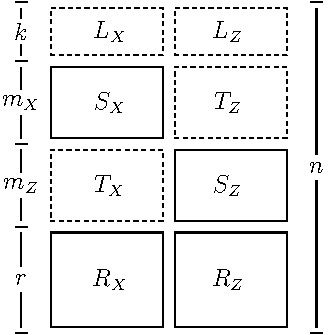
\includegraphics[]{pic-symplectic.pdf}
\end{center}
The solid rectangles indicate operators that
span the $X$ and $Z$ parts of the gauge group,
and the dashed rectangles indicate operators that
do not live inside the gauge group.

We consider each of these blocks 
$L_X, L_Z, S_X, T_Z, T_X, S_Z, R_X, R_Z,$
as well as $G_X,G_Z,$
%Each of these blocks can be thought of as 
as either a set of $\Fnd$ vectors (the rows) or as an 
$\Field$-linear operator.
For example, we write $u\in R_X$ to mean $u$ is 
a row of the matrix $R_X$.
%As an $r\times n$ matrix this operator is
%$$
%    R_X : \Field^n] \to \Field^r]
%$$
%Given $v\in \Fr$ then $u = v R_X$ is
%a generic vector in the rowspace of $R_X.$

We first find the stabilizers $S_Z$.
These are built out of $\Fnd$ vectors from the span of $G_Z$
that commute with the rows of $G_X:$
\begin{align*}
    \Span{S_Z} &= \{\  vG_Z \ |\  v G_Z G_X^\top = 0, \ \ v \in F_{|G_Z|}\ \} \\
               &= \{\  vG_Z \ |\  v^\top \in \Ker(G_X G_Z^\top)  \ \}.
\end{align*}
The generators (rows of $S_Z$) are then extracted
from this span by row reduction.
We swap the role of $X$ and $Z$ to find $S_X.$

Once we have the stabilizers, in order to
complete the above table as a presentation
of the Pauli group we solve the
following $\Field$-linear block matrix equation,
%All of this can be summarized in the block matrix equation:
$$
\left( \begin{array}{l}
L_X\\
S_X\\
T_X\\
R_X
\end{array} \right)
\left( \begin{array}{l}
L_Z\\
T_Z\\
S_Z\\
R_Z
\end{array} \right)^\top =
I,
$$
%And once again we have a presentation of the Pauli group.
subject to the restriction that the rows of
$R_X$ lie in the span of $G_X$ and
the rows of $L_X$ do not.
Similarly for $R_Z$ and $L_Z.$
This set of 16 equations is quadratic in the unknown variables
and so it is not obvious how to proceed, but it turns out a
systematic way can be found.

We begin by finding $L_Z.$
These operators satisfy the following \emph{homology} condition:
$$
    l_Z \in L_Z \smbox{is given by} l_Z^\top \in \Ker(G_X) \smbox{mod} \Span{S_Z}.
$$
In other words, $L_Z$ is formed from a basis for the kernel of $G_X$ 
row-reduced using $S_Z.$
To be more specific %about this operation of mod $\Span{S_Z}$
we take any direct sum decomposition
$$\Fnd = \Span{S_Z} \oplus V$$
then the operation of mod $\Span{S_Z}$ is the
projection onto $V.$
We can explicitly write such a 
projector as the $n\times n$
matrix given by
$$
    P_Z = I + A^\top S_Z
$$
where the matrix $A$ is the $m_Z\times n$ matrix consisting of
the leading 1's in any row-reduction of $S_Z.$
We define $P_X$ similarly for the operation of mod $\Span{S_X}.$

To find $L_X$ we solve the following $\Field$-linear
system:
%\begin{align*}
%    L_Z L_X^\top &= I, \\
%    G_Z L_X^\top &= 0.
%\end{align*}
$$
\left( \begin{array}{l}
L_Z\\
G_Z\\
\end{array} \right)
L_X^\top = 
\left( \begin{array}{l}
I\\
0
\end{array} \right)
$$

The reduced gauge group matrix $R_X$
is found as a row-reduction of $G_X P_X.$
We cannot merely set $R_Z$ to be $G_Z P_Z$ 
because we also require $R_X R_Z^\top = I.$
Instead we define the auxiliary matrix
$\widetilde{R}_Z$ to be a row-reduction of  $G_Z P_Z.$

The error operators $T_X$ are then found as the solution
to the $\Field$-linear system:
%\begin{align*}
%    S_Z T_X^\top &= I,\\
%    L_Z T_X^\top &= 0,\\
%    \widetilde{R}_Z T_X^\top &= 0.
%\end{align*}
$$
\left( \begin{array}{l}
L_Z\\
S_Z\\
\widetilde{R}_Z
\end{array} \right)
T_X^\top = 
\left( \begin{array}{l}
0\\
I\\
0
\end{array} \right)
$$
And then the operators $T_Z$ solve the $\Field$-linear system:
%\begin{align*}
%    S_X T_Z^\top &= I,\\
%    T_X T_Z^\top &= 0,\\
%    L_X T_Z^\top &= 0,\\
%    R_X T_Z^\top &= 0.
%\end{align*}
$$
\left( \begin{array}{l}
L_X\\
S_X\\
T_X\\
R_X
\end{array} \right)
T_Z^\top = 
\left( \begin{array}{l}
0\\
I\\
0\\
0
\end{array} \right)
$$
Finally at this point $R_Z$ is given as the solution to
%\begin{align*}
%    R_X R_Z^\top &= I,\\
%    L_X R_Z^\top &= 0,\\
%    S_X R_Z^\top &= 0,\\
%    T_X R_Z^\top &= 0.
%\end{align*}
$$
\left( \begin{array}{l}
L_X\\
S_X\\
T_X\\
R_X
\end{array} \right)
R_Z^\top = 
\left( \begin{array}{l}
0\\
0\\
0\\
I
\end{array} \right)
$$
Note that $R_Z$ and $\widetilde{R}_Z$ have identical span 
and so we have $R_Z T_X^\top = 0.$

We call this array of eight $\Field$-linear 
matrices
an $(L,S,T,R)$-decomposition of the gauge group.
In general this will not be unique for
any given gauge group.

\subsection{The Hamiltonian}

The complex Hilbert state space of our
Hamiltonian has $2^n$ dimensions and we
write this space as $\Complex[2^n]$.
This notation is meant to suggest that
we are forming a $\Complex$ vector space
using $2^n$ ``points'' 
as basis vectors.
Working in the computational basis,
we do indeed have $2^n$ such points; 
these are the elements of $\Fnd.$
And so we make the identification
$$
    \Complex[2^n] \cong \Complex[\Fnd].
$$
In other words, we are labeling 
our basis vectors with elements of $\Fnd$
and therefore such notation as
$$
    \bra{u} H \ket{v}
$$
with $u, v \in \Fnd$ makes sense.
We will make further use of this below,
by writing  $\Field$-vector space 
computations inside the Dirac brackets.

Returning to the code $(L,S,T,R)$-decomposition
above,
given the Pauli operator $t\in T$ such that $t = t_X t_Z$ (in $\Pauli_n$)
we get a basis for the irrep $\rho_t$:
$$
    \{ \ket{v R_X + t_X} \ \mbox{such that}\  v \in \Frd \}.
$$
In other words,
the basis of the irrep $\rho_t$ is 
an affine subspace of $\Fnd.$
Each such affine subspace is indexed by an
element of $\Frd$ and
all of these are
translates of each other,
so we make the following identification:
$$
\Complex[\{vR_X+t_X\}_{v\in\Frd}]
\cong \Complex[\Frd].
$$
This will allow us to write the components
of each block $H_t$ of the Hamiltonian
as $\bra{u}H_t\ket{v}$ for $u,v\in\Frd.$
We make this identification of affine subspaces
not out of laziness but because it will
help us to compare each of
the Hamiltonian blocks $H_t$ below.
\danbrowne{I'd suggest you introduce Ht and Htx,tz more prominently. }

\begin{framed}
\noindent{\bf Important:}
The computational basis identifies
basis vectors of $\Complex[2^n]$
with elements of a finite vector space $\Fnd$:
$$
    \Complex[2^n] \cong \Complex[\Fnd].
$$
The $(L,S,T,R)$-decomposition naturally
decomposes $\Fnd$ into $2^{m_Z+k}$ affine subspaces:
$$
    \{ v R_X + t_X + l_X \}_{v\in\Frd}
$$
for each $t_X \in \Span{T_X}, l_X \in \Span{L_X}.$
Each such affine subspace forms a basis
for the irreducible blocks $H_{t_X,t_Z}$ of $H$,
and can be naturally identified with $\Frd:$
$$
    H_{t_X,t_Z} : \Complex[\Frd] \to \Complex[\Frd].
$$
\end{framed}

We now wish to understand the action of the
gauge group on each of its irreps.
Starting with the $t_X,t_Z=0,0$ irrep,
this is where each of the stabilizers has
a trivial action. 
In $\Fn$ this
corresponds to the additive action of the zero vector.

\newcommand{\pluseq}{\mathrel{+}=}
States $u\in\Span{R_X}$ can be built from a
vector matrix product
$$
    u = v R_X
$$
with $v\in\Frd.$
Since $R_X R_Z^\top = I$
we can write $v = u R_Z^\top.$
Each $g_X\in G_X$ acts on $u$ to give
\begin{align*}
    u_1 &= (u + g_X) \ \mbox{mod}\ \Span{S_X} \\
        &= (u + g_X) P_X \\
        &= (v R_X + g_X) P_X.
\end{align*}
writing $u_1 = v_1 R_X$ we then have
\begin{align*}
    v_1 &= (v R_X + g_X) P_X R_Z^\top \\
        &= v + g_X R_Z^\top.
\end{align*}
%\todo{XXX explain that \todo{$P_X R_Z^\top = R_Z^\top$} etc. XXX}
So we have that working in the computational
basis, the action of the $X$ part of the
gauge group in the $t_X,t_Z=0,0$ irrep is to send
%$v\in R_X$ to 
$v\in \Frd$ to $v + g_X R_Z^\top.$
In summary, we have the following contributions from the
$G_X$ terms of the Hamiltonian:
$$
%    H_{0,0}(v, v+g_X  R_Z^\top) \ne 0,\ \ \mbox{for}\ g_X\in G_X, v\in \Frd
    \bra{v} H_{0,0} \ket{v+g_X  R_Z^\top} 
        \pluseq 1,\ \ \mbox{for}\ g_X\in G_X, v\in \Frd
$$
where we use the $\pluseq$ notation
because there may be other contributions to the
same component.
These terms will always be off
the diagonal unless $g_X$ is a stabilizer.

The action of the $G_Z$ gauge group
contributes to the diagonal of $H.$
These diagonal terms apply a kind of
``potential energy'' penalty
to the basis states
that depends on the \emph{syndrome} vector:
$$
    \mbox{syndrome}(u) = G_Z u^\top
$$
for $u^\top \in \Fn.$
This is an $\Field$-vector that has one component for
each row of $G_Z.$
Writing $|G_Z|$ for the number of these rows, and 
using a \emph{weight} function $w$ that just counts
the number of non-zero entries in any $\Field$-vector
we have the following contributions to
the Hamiltonian:
$$
    \bra{v} H_{0,0} \ket{v} 
        \pluseq |G_Z| - 2w(G_Z R_X^\top v^\top),
$$
for $v\in \Frd.$

Adding up all of the above we
have in summary,
$$
H_{0,0} = \sum_{\substack{v\in\Frd\\g_X\in G_X } }
  \ket{v+g_X  R_Z^\top}\bra{v} 
  + \sum_{v\in\Frd} \bigl(|G_Z| - 2w(G_Z R_X^\top v^\top)
    \bigr) \ \ket{v}\bra{v}.
$$

For any $t_X\in \Span{T_X}$ the Hamiltonian block $H_{t_X,0}$
has components indexed by basis vectors:
$$
    u = v R_X + t_X
$$
this means that the $G_X$ gauge terms
have the same effect on $H_{t_X,0}$
as $H_{0,0}$ and only the diagonal has changed:
$$
H_{t_X,0} = \sum_{\substack{v\in\Frd\\g_X\in G_X } }
  \ket{v+g_X  R_Z^\top}\bra{v} 
  + \sum_{v\in\Frd} \bigl(
    |G_Z| - 2w(G_Z R_X^\top v^\top + G_Z t_X^\top)
    \bigr) \ \ket{v}\bra{v}.
$$
%Writing the difference explicitly:
%$$
%    H_{0,0} - H_{t_X,0} = 
%  \sum_{v\in\Frd} 2\bigl(
%    w(G_Z R_X^\top v^\top + G_Z t_X^\top)
%    -w(G_Z R_X^\top v^\top)
%    \bigr) \ \ket{v}\bra{v}.
%$$
The general form of
each Hamiltonian block is:
%\begin{align*}
%H_{t_X,t_Z} = &\sum_{\substack{v\in\Frd\\g_X\in G_X } }
%    \eta(t_Z g_X^\top)
%  \ \ket{v+g_X  R_Z^\top}\bra{v} \\
%  &+ \sum_{v\in\Frd} \bigl(
%    |G_Z| - 2w(G_Z R_X^\top v^\top + G_Z t_X^\top)
%    \bigr) \ \ket{v}\bra{v}.
%\end{align*}
\begin{equation}\label{hamiltonian}
H_{t_X,t_Z} = \sum_{\substack{v\in\Frd\\g_X\in G_X } }
    \eta(t_Z g_X^\top)
  \ \ket{v+g_X  R_Z^\top}\bra{v} 
  + \sum_{v\in\Frd} \bigl(
    |G_Z| - 2w(G_Z R_X^\top v^\top + G_Z t_X^\top)
    \bigr) \ \ket{v}\bra{v}.
\end{equation}
Here we use $\eta$ to send 
$t_Zg_X^\top$ which is an $\Field$ value
to the multiplicative subgroup $\{\pm1\}$
of $\Complex:$
$$
    \eta(0) = 1,\ \eta(1) = -1.
$$
The $\eta(t_Zg_X^\top)$ term
is a kind of parity check that
picks up one phase flip for (some of)
the $X$ type stabilizers found in $g_X.$
This works because $T_Z$ is a left inverse
of $S_X^\top.$
The $t_Z\in\Span{T_Z}$ selects which
$X$ type stabilizers act as $-1$ in this irrep.

In summary, we have the complete representation
theory for $CSS$ gauge code Hamiltonians.
%It is a remarkable fact that this involves such
%a close interplay with $\Field$ linear algebra.


%%%%%%%%%%%%%%%%%%%%%%%%%%%%%%%%%%%%%%%%%%%%%%%%%%%%%%%%%%%%%%%%%%%%%%%%%%%%%%%
%

\section{Gapless 1D models}

In this section we briefly introduce two important
one dimensional models that fit into the CSS gauge code framework.

The $XY$-model \cite{Pfeuty1970}
lives on a one dimensional chain of $n$ qubits.
We write the gauge group generators as
$$
    G_0 = \{ X_i X_{i+1}, Z_i Z_{i+1}\ \ \mbox{for}\ \ i=1,...,n \}
$$
with periodic boundary conditions.
For $n$ even this model has no logical operators, one 
$X$-type stabilizer and one $Z$-type stabilizer.
With $n$ odd, there are no stabilizers and $k=1.$
Normally the gauge operators are written as 
$\{ X_i X_{i+1}, Y_i Y_{i+1} \ \mbox{for}\ i=1,...,n \}$
but note that there is an automorphism of the Pauli group
that sends $G_0$ to these operators.
For $n$ even, this model is exactly solvable,
and the gap goes to zero
as the system size grows \cite{Lieb1961}.

For the one dimensional transverse field
Ising model, we have 
$$
    G_0 = \{ X_i, Z_i Z_{i+1}\ \ \mbox{for}\ \ i=1,...,n \},
$$
with periodic boundary conditions.
This model has one 
$X$-type stabilizer and no logical operators.
This model is also exactly solvable, with gap going to zero
as the system size grows \cite{Pfeuty1970}.

\section{Perron-Frobenius theory}

\danbrowne{You need to make it clearer how much of this is newly defined and how much is developing previous work. Is the Perron-Frobenius construction your own?}

%We restrict our attention to Hamiltonians whose off-diagonal entries
%are non-negative (in some basis).
%These are also known as \emph{stoquastic} Hamiltonians \cite{Bravyi2006}.
%This can be achieved by considering Hamiltonians where each term
%involves either $X$-type operators or $Z$-type operators but not both.
%That is, $G_0$ consists only of $X$-type operators and $Z$-type operators.
%We will call this a \emph{CSS gauge code Hamiltonian} after the stabilizer codes
%of the same name.
%We also shift the Hamiltonian by a constant energy, so that
%the diagonal entries are non-negative:
%$$
%%\Ham := \sum_{g\in G_0} \rho_{\mathrm{pauli}}(g).
%\Ham := \sum_{g\in G_0} \rho_{\mathrm{pauli}}(g) + kI.
%$$
%This does not change the spectral gap or eigenvectors.

%This is another kind of representation theory of $\Pauli_n.$
%We are representing either $G_X$ or $G_Z$ as a permutation representation (?)
%It has the ability to extract irreps of $G$ corresponding to
%the $X$ type operators as affine subspaces $\{vR_X+t\}$ of $\Fn.$
%For the $Z$ representations we will still need the complex
%representation theory to build states on $\Complex[\{vR_X+t\}]$
%that look like ``waves''.
%These (stationary) waves do indeed have a geometric interpretation,
%with the wavefront nodes being identified with so-called Cheeger cuts.
%To switch back and forth between the $X$ and $Z$ type
%representations 

%We begin this section with the following two definitions.
A CSS gauge code is \emph{self-dual} when the $X$ and $Z$ type
gauge generators are equal: $$G_X = G_Z.$$
The $XY$-model is an example of a self-dual CSS gauge code.
A CSS gauge code is \emph{weakly self-dual}
when there is a permutation $P$ on the set of $n$ qubits
that induces equality of the gauge generators:
$$
    G_X P = G_Z,
$$
where we write $P$ as an $n\times n$ permutation matrix.
The compass model is then weakly self-dual when we transpose
the square lattice of $l\times l$ qubits.

Any stabilizer that acts as $-1$ in a given block of
the Hamiltonian we will call a \emph{frustrated stabilizer}
(with respect to the given block.)
Similarly, a \emph{satisfied stabilizer} acts as $+1$ in a given
block of the Hamiltonian.
We will call a
vector \emph{stabilized} if it is a $+1$ eigenvector 
of every stabilizer in the given gauge group.

We now turn to another notion of reducibility, coarser than
the group theoretic reducibility.
One way to understand this is via graph theory.
Given a CSS gauge code Hamiltonian $H,$ 
we see that 
the diagonal terms (working in the computational basis)
come from the $Z$ operators and the off-diagonal terms
come from $X$ type operators.
We think of the $Z$ operators as potential energy, and the
$X$ operators as kinetic terms.
This suggests the following definition.
We define a graph $\Gamma$ with vertices the $2^n$ computational
basis elements, and edges:
$$
    \ket{v} \mapsto g_X \ket{v}, \smbox{for all} v\in\Fnd, g_X\in G_X.
$$
These are undirected edges because $g_X^2 = I.$
We also add weighted loops corresponding to the $Z$-type gauge operators:
$$
    \ket{v} \mapsto \sum_{g_Z\in G_Z} g_Z \ket{v}, \smbox{for all} v\in\Fnd.
$$
In this way we can consider $H$ and $\Gamma$ interchangeably,
as either a matrix or a graph.
An irreducible matrix is one whose corresponding graph is connected.
The examples with diagrams in section 2.1.1 are meant to illustrate this
graph picture.

The off-diagonal entries of $H$ are all positive.
If we use a spectral shift operator, a constant multiple of the identity $+cI$,
we find that $H+cI$ is a non-negative matrix. 
We call such a matrix \emph{Stoquastic} \cite{Bravyi2008}.

\dolemma{2.1}
\todo{Given a ...}
The matrix $\Gamma$ decomposes into irreducible
stoquastic matrices $\Gamma_{t_X}$ 
indexed by $t_X\in\Span{T_X}$
with multiplicity $2^k$:
$$
    \Gamma = \bigoplus_{
    \substack{t_X\in\Span{T_X}\\l_X\in\Span{L_X}}}
        \Gamma_{t_X}.
$$

\doproof
We identify the computational basis with
the elements of $\Field_n.$
As a graph, $\Gamma$ has edges starting from $\ket{v}$
that are given by
$$
\ket{v} \mapsto g \ket{v}, \smbox{for} v\in\Fnd, g\in G_X.
$$
This means that paths starting from $\ket{v}$ are given by
products $g_i...g_1$ of the elements of the group $G_X:$
$$
    \ket{v} \mapsto g_1 \ket{v} \mapsto ... \mapsto g_i...g_1 \ket{v}
$$
Switching to the additive $\Field_n$ notation, we
therefore have that $\ket{v}$ and $\ket{u}$ are in the
same component of $\Gamma$ iff $u = v+g$ for some $g\in\Span{G_X}.$
%We write $\Gamma_0$ for the component of the vector $\ket{0}$
The vectors
$$\{ \ket{t_X + l_X} \}_{t_X\in\Span{T_X}, l_X\in\Span{L_X}}$$
of $\Gamma$ 
\tombstone

%Using the $\Field$-linear $(L,S,T,R)$-decomposition of the gauge group
%we then have the following:
%\begin{framed}
%\noindent In the computational basis, any CSS gauge code
%Hamiltonian $H$ is the direct sum of $2^{m_Z}$
%irreducible matrices $\Gamma_{t_X}$
%indexed by $t_X\in\Span{T_X}$
%with multiplicity $2^k$:
%$$
%    H = \bigoplus_{
%    \substack{t_X\in\Span{T_X}\\l_X\in\Span{L_X}}}
%        \Gamma_{t_X}.
%$$
%\end{framed}

%See \cite{Baez2012}
%We return to the investigation of Hamiltonians
%formed from CSS gauge codes.
%We can think of such Hamiltonians as the adjacency matrix of a graph.
%Loosely speaking we can view the off-diagonal terms as 
%raising and lowering operators, and the diagonal
%terms measure the energy of each level.

%Now we invoke the Peron-Frobenius theorem.
%Each of the blocks $\Gamma_{t_X}$ is also Perron-Frobenius
%and in combination with their irreducibility, the Perron-Frobenius
%theorem gives:

\dolemma{2.2}
\todo{Given a ...}
For each $t_X\in\Span{T_X}$
the largest eigenvalue 
of $\Gamma_{t_X},$
$\lambda_1(\Gamma_{t_X})$
is non-degenerate,
and is associated with an eigenvector 
$v_1(\Gamma_{t_X})$
with positive components.

\doproof
By the previous Lemma, 
we can apply the  Perron-Frobenius theorem
to the matrices $\Gamma_{t_X}$.
\tombstone

A basis for each $\Gamma_{t_X}$ is given by a coset
of $G_X$ in $\Fnd:$
$$
    \bigl\{ \ket{v S_X + u R_X + t_X} \bigr\}_{v\in \Field_{m_X}, u\in\Frd}.
$$



\dolemma{2.3}
For any gauge code Hamiltonian $H$,
every groundstate of $H$ is stabilized.

\doproof
%Our goal will be to show that the
%groundspace of $H$ is spanned
%by vectors which are stabilized.
%To begin, let $v_1$ be the top
%eigenvector of $\Gamma_{t_X}$ with $t_X\in\Span{T_X}.$
%Because $v_1$ has all positive components
%it will be fixed by  any operator
%$s\in\Span{S_Z}$.
%To show that the $X$ type stabilizers
%also fix $v_1$ 
%we use weak self-duality
%and see that by change of basis
%we can swap the roles of the $X$ and $Z$ type operators.
We will construct a basis for the groundspace consisting of
vectors that are stabilized.
The set of top eigenvectors 
$$
    \{ v_1(\Gamma_{t_X}) \}_{t_X\in\Span{T_X}}
$$
must contain a basis for the groundspace of $H.$
Let such a basis vector be $v_1(\Gamma_{t_X})$ for some $t_X.$
This vector is positive by Lemma 2.2.
We have the commutativity
$$
    \Gamma_{t_X} s = s \Gamma_{t_X}
$$
for any $s\in S_X.$
\todo{why?} 
Therefore $\ket{v_1}$ is an eigenvector for every $X$-type
stabilizer, but the eigenvalue must be $+1$ because any
$X$-type operator acts by permuting basis elements and
$\ket{v_1}$ is positive.

We have that
$$
    \Gamma_{t_X} = \bigoplus_{t_Z\in\Span{T_Z}} H_{t_X,t_Z}
$$
\todo{why?} 
and so $\ket{v_1}$ must be an eigenvector of
the $Z-$type stabilizers.
Using \Eref{hamiltonian}
we have that 
\begin{align*}
    \Gamma_{0} - \Gamma_{t_X}
    &= \sum_{t_Z\in\Span{T_Z}} H_{0,t_Z} - H_{t_X,t_Z} \\
    &= \sum_{t_Z\in\Span{T_Z}} G_z t_X^\top \sum_{u\in\Field_r} \ket{u}\bra{v}
\end{align*}
\todo{basis fail}
And therefore, if $t_X\ne 0:$
$$
    \bra{v_1} \Gamma_0 \ket{v_1} > \bra{v_1} \Gamma_{t_X} \ket{v_1}
$$
so we must have that $t_X=0$. Therefore 
$\ket{v_1}$ is stabilized by the $Z-$type stabilizers.
\tombstone

\doproposition{2.4}
For any weakly self-dual gauge code Hamiltonian $\Ham$
we have:
$$\lambda_1(\Ham) = \lambda_1(\Ham_{0,0})$$
and for $t_X\in\Span{T_X}, t_Z\in\Span{T_Z}$
with $t_X\ne 0$ or $t_Z\ne 0$,
$$
\lambda_1(\Ham) > \lambda_1(H_{t_X,t_Z}).
$$

\doproof
Consequence of previous lemma.
\tombstone

%\danbrowne{This is a key result and you speed through it too quickly. Can you write this as a lemma with a formal proof?}

Notice that 
$H_{0,0}$ is also irreducible stoquastic (in the computational basis)
and so has non-degenerate
groundspace, but it appears with multiplicity $2^k$ within
the Hamiltonian $H$ and this accounts for the degeneracy of the
groundspace of $H$.

%Taken together, these eigenvectors form a basis for the
%groundspace of the system.
%Stabilizers act as $+1$ or $-1$ on eigenvectors
%of the Hamiltonian.
%A stabilizer $s\in\Pauli^X$ just permutes the
%coordinates of the groundstate and so must fix any
%groundstate. 
%A stabilizer $s\in\Pauli^Z$ acts trivially
%on $\ket{0...0}$ and therefore must also fix any groundstate.
%We have demonstrated the following

%A simple variational argument % ???
%shows that the top eigenvector (the groundstate)
%can be chosen to have all positive entries
%(this is the Perron-Frobenius theorem)
%and therefore is stabilized:

The next goal is to search for
the second eigenvalue of $H$,
$\lambda_2(H).$

%Using a basis change and the
%above equation for $H_{t_X,0}$
%we have
%\begin{framed}
%\noindent{\bf Fact 2:}
\dolemma{2.5}
Given a 
gauge code Hamiltonian $\Ham$ and
$t_X\in \Span{T_X},$
the blocks $\Ham_{t_X,0}$ 
are stoquastic.

\doproof
because why?
\tombstone


\doproposition{2.6}
For a weakly self-dual gauge code Hamiltonian $H$,
\begin{align*}
\lambda_1(\Ham_{t_X,0}) &< 
    \lambda_1(\Ham_{t_X,t_Z}) \ \smbox{and}\\
\lambda_1(\Ham_{0,t_Z}) &< 
    \lambda_1(\Ham_{t_X,t_Z}),
\end{align*}
where $t_X\ne 0$ and $t_Z\ne 0.$

\doproof
because why?
\tombstone

%\danbrowne{Please spell out the argument more clearly. It isn't immediate that this follows from your two facts. }
Therefore,
to find the spectral gap of a weakly self-dual gauge code Hamiltonian,
%which is the difference of the top two eigenvalues of the Hamiltonian,
we need only examine the top two eigenvalues of $H_{0,0}$ and 
the top eigenvalue of $H_{t_X,0}$ for each $t_X\in T_X.$ 
We summarize this in the theorem:

\dotheorem{2.7}
For a weakly self-dual gauge code Hamiltonian $H$,
the spectral gap is given by:
$$
    \min \bigl\{ \lambda_1(H_{0,0}) - \lambda_2(H_{0,0}),
        \min_{t_X\in\Span{T_X}} 
         \{ \lambda_1(H_{0,0}) - \lambda_2(H_{t_X,0}) \} \bigr\}
$$
\doproof
Combine Proposition 2.4 with Proposition 2.6.
\tombstone


\section{The gauge color code model}

%\begin{center}
%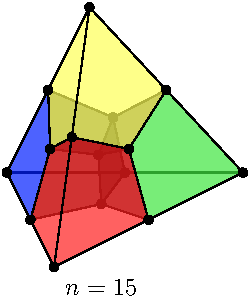
\includegraphics[width=0.3\columnwidth]{pic-gcolor-1.pdf}
%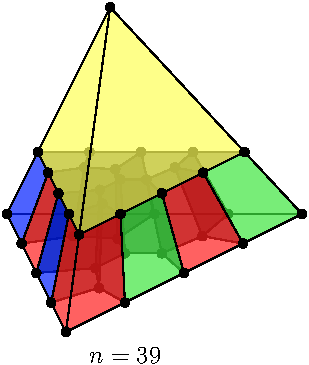
\includegraphics[width=0.3\columnwidth]{pic-gcolor-15.pdf}
%\end{center}
%
%\begin{center}
%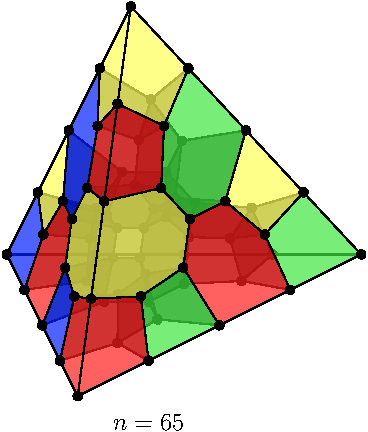
\includegraphics[width=0.3\columnwidth]{pic-gcolor-2.pdf}
%\end{center}

We now turn to the central animal that motivated
the theory developed in this chapter.

The three dimensional gauge color code \cite{Bombin2015,Bombin2015single,Kubica2015}
is a self-dual CSS gauge code. 
It is based on the following geometric construction known
as a \emph{colex} \cite{Bombin2007exact}.
We begin with a tetrahedron and subdivide it into finitely many
convex 3-dimensional polytopes, or \emph{bodies}.
Each body has a boundary consisting of 0-dimensional cells
which we call \emph{vertices}, 1-dimensional cells called \emph{edges}
and 2-dimensional cells called \emph{faces}.
By a \emph{cell} we mean any of these 0,1,2 or 3-dimensional convex polytopes.
Any two bodies in this tetrahedral subdivision will
have either empty intersection or otherwise intersect
on a common vertex, edge or face.
When the intersection is on a face these two bodies
are called \emph{adjacent}.
Two vertices in the same edge will also be called adjacent.
Each body is colored by one of four \emph{colors},
either taken to be red, green, blue, yellow or 
otherwise an element of the set $\{1, 2, 3, 4\}.$
The four exterior triangular faces of the bounding tetrahedron are
called \emph{regions,} the intersection of two regions is called
a \emph{border} and the intersection of three regions is called
a \emph{corner.}
A cell not contained within any region is called an interior cell.

This colored cellulation is required to have the following further properties:
\begin{enumerate}
\item Adjacent bodies have different colors.
\item Each region has a unique color 
such that no bodies intersecting that region has that color.
\item All vertices are adjacent to four other vertices,
except for the corner vertices which are adjacent to three other vertices.
\end{enumerate}

Here we show some instances of this construction,
along with the colors of the unobscured bodies.
Each instance is labeled by the number of vertices $n$.
\begin{center}
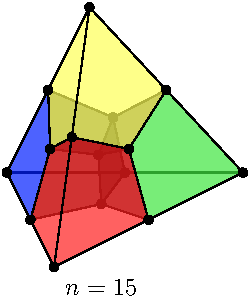
\includegraphics{pic-gcolor-1.pdf}\ \ \ \ \ \ \ \ \ \ \ 
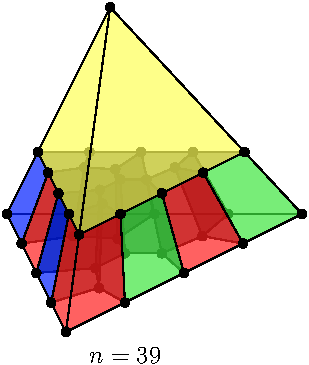
\includegraphics{pic-gcolor-15.pdf}
\end{center}

\begin{center}
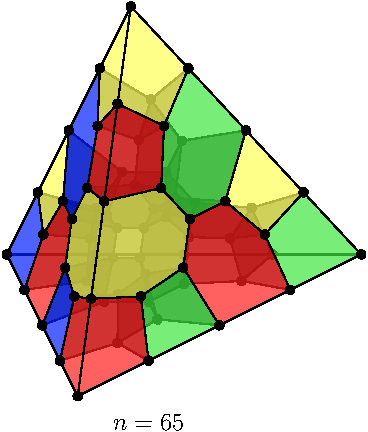
\includegraphics{pic-gcolor-2.pdf}\ \ \ \ \ \ \ \ \ \   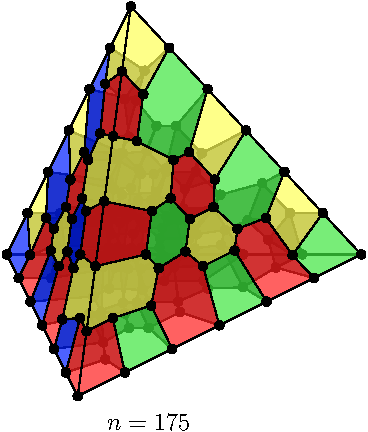
\includegraphics{pic-gcolor-3.pdf}
\end{center}

%From the above conditions it follows that:\\
We note the following consequences of the above conditions.
Every face supports an even number of vertices.
% Each face cobounds two bodies, the other bodies that
% share an edge must be 2-colorable, ie even number of edges.
We now think of each region as corresponding to a ``missing'' body.
Each edge is then contained in the boundary of three bodies.
%Every interior edge is in the boundary of three bodies.
%Edges contained in the regions are either in the boundary of two bodies or
%otherwise are contained in one of the borders and the boundary of one body.
This means we can associate a unique color to each edge,
which is also the color of two bodies intersecting a vertex of the edge.
That is, each edge joins two bodies of the same color.
Each face bounds two bodies, and so we color each face with the two colors of these bodies.
%We color each face with the two colors of the bodies 

Using this cellulation we now construct the gauge code.
Qubits are associated with the $n$ vertices.
We associate operators to other cells, or union of cells,
by using the contained vertices as support.
\danbrowne{Is this correct? All the operators here are built from faces, not cells. }
Because this is a self-dual code, the same goes for
both the $X$ and $Z$ type operators.
%and we confuse the distinction between union of cells
%and the corresponding $X$ or $Z$ type operator.
The $X/Z-$type gauge group is generated by
$X/Z-$type operators supported on each face.
The $X/Z-$type stabilizer group is generated by
$X/Z-$type operators supported on each body.
There is one $X/Z-$type logical operator and these
are generated by
$X/Z-$type operators supported on any region.

%%%%%%%%%%%%%%%%%%%%%%%%%%%%%%%%%%%%%%%%%%%%%%%%%%%%%%%%%%%%%%%%%%%%%%%%%%%%%%%
%


\section{The orbigraph}

Performing numerics on small gauge code models makes
it evident that there is a great deal more symmetry than
we have found using the above techniques.
In particular, the components of eigenvectors 
have many identical values.
This motivates the following exploration of the symmetry 
of the Hamiltonian.

\def\auto{\mathcal{A}}

A \emph{graph automorphism} is a permutation matrix $P$
such that 
$$P^T \Ham P = \Ham.$$
The set of all such graph automorphisms 
form a group $\auto$.
The goal here is to find eigenvectors of $H$ that are
invariant under the action of $\auto.$
Such an eigenvector will have components that
are constant on the orbits of $\auto,$
so therefore it will live naturally on the
vector space whose basis is these orbits.
We can do better than this, and actually 
project the graph itself down onto this space.
We do this by constructing a new graph
which we call the \emph{orbigraph}.
%form a group $\auto(H)$ or just $\auto$ when the graph is understood.
%We now define a new matrix $\Ham/\auto$
The matrix for the orbigraph is written $\Ham/\auto$
and acts on the vector space with basis consisting
of the orbits of $\auto.$
It follows that the components of $\Ham/\auto$,
indexed by a pair of $\auto-$orbits $i$ and $j$, is defined by
$$
    (\Ham/\auto)_{ij} = |\{ g\in G \smbox{s.t.} gv \in j \}| \smbox{where}v\in i.
$$
In other words, 
$(\Ham/\auto)_{ij} $ counts the number of gauge group
elements that sends any particular element $v$ of the 
$\auto-$orbit $i$ to the $\auto-$orbit $j.$

Here is a simple example. % potential only depends on hamming weight: Jarret
We take as gauge group 
$$G = \{XII, IXI, IIX, ZII, IZI, IIZ\}.$$
The Hamiltonian $H = \sum_{g\in G} g$ has matrix:
$$
H = \left(\begin{array}{rrrrrrrr}
 3 &  1 &  1 &  1 &  . &  . &  . &  . \cr
  1 &  1 &  . &  . &  1 &  1 &  . &  . \cr
  1 &  . &  1 &  . &  1 &  . &  1 &  . \cr
  1 &  . &  . &  1 &  . &  1 &  1 &  . \cr
  . &  1 &  1 &  . & -1 &  . &  . &  1 \cr
  . &  1 &  . &  1 &  . & -1 &  . &  1 \cr
  . &  . &  1 &  1 &  . &  . & -1 &  1 \cr
  . &  . &  . &  . &  1 &  1 &  1 & -3
\end{array}\right)
$$
where we indicate zero entries with a dot.
In this case, the automorphism group is $\auto=S_3,$
there are four $\auto-$orbits, and
$$
H/\auto = \left(\begin{array}{rrrr}
 3 &  3 &  . &  . \cr
  1 &  1 &  2 &  . \cr
  . &  2 & -1 &  1 \cr
  . &  . &  3 & -3
\end{array}\right).
$$
In this case the automorphism group $\auto$ of the graph
is the same as the automorphism group $Aut(G)$ of the gauge group,
but in general it is possible that $Aut(G) < \auto.$

Note that the orbigraph is no longer Hermitian,
and in general will not even be normal.

We can also write $H/\auto = QHP$ using the following two matrices for $P$ and $Q:$
$$
Q = 
\left(\begin{array}{rrrrrrrr}
 1 &  . &  . &  . &  . &  . &  . &  . \cr
  . &  1 &  . &  . &  . &  . &  . &  . \cr
  . &  . &  . &  . &  1 &  . &  . &  . \cr
  . &  . &  . &  . &  . &  . &  . &  1
\end{array}\right),\ \ \ 
P = 
\left(\begin{array}{rrrr}
 1 &  . &  . &  . \cr
  . &  1 &  . &  . \cr
  . &  1 &  . &  . \cr
  . &  1 &  . &  . \cr
  . &  . &  1 &  . \cr
  . &  . &  1 &  . \cr
  . &  . &  1 &  . \cr
  . &  . &  . &  1
\end{array}\right).
$$
The idea is that each column of $P$ sums over an orbit,
and each row of $Q$ chooses one member of each orbit.
%See also \cite{Cvetkovic1980} chapter 5.

%The automorphisms of the gauge group, $Aut(G)$ will induce an
%automorphism of the graph by \todo{XXX}...
%In particular, elements of the stabilizer group $\Stab$ induce graph 
%automorphisms by \todo{XXX}...
%In general there may be more symmetry in the graph that
%we cannot access via a group automorphism.

In general, we will apply this idea to each of the blocks $H_{t_X,0}$.
From {\bf Fact 2} above, and using the fact that we are
summing over a trivial representation of $\auto$ we have the following:
\begin{framed}
\noindent{\bf Fact 3:}
The spectrum of the orbigraph of $\Ham_{t_X,0}$ contains the ground eigenvalue of $\Ham_{t_X,0}.$
\end{framed}
\danbrowne{Please prove this.}

%%%%%%%%%%%%%%%%%%%%%%%%%%%%%%%%%%%%%%%%%%%%%%%%%%%%%%%%%%%%%%%%%%%%%%%%%%%%%%%
%
\subsection{The compass model}
For the next example we take the $l=3$ compass model.
$\Ham_{0,0}$ acts on a 16 dimensional space.
The order of $\auto$ is $72$, and we find three $\auto-$orbits.
% This time $Aut(G) = \auto$ ???
The orbigraph method can be applied in the case
where the Hamiltonian weights for $X$ and $Z$ are uniform as $w_X$ and $w_Z.$
We separate the $X$ and $Z$ terms of the orbigraph to show
how this works:
$$
\Ham_{0,0}/\auto = 
\left(\begin{array}{rrr}
 . &  9 &  . \cr
  1 &  4 &  4 \cr
  . &  6 &  3
\end{array}\right) + 
\left(\begin{array}{rrr}
 9 &  . &  . \cr
  . &  1 &  . \cr
  . &  . &  -3
\end{array}\right)
=
\left(\begin{array}{rrr}
 9 &  9 &  . \cr
  1 &  5 &  4 \cr
  . &  6 &  .
\end{array}\right)
$$
This can be solved analytically and we find $\lambda_1 = 4+2\sqrt{13} \cong 11.21110255.$
Keep in mind that the original state space has dimension $2^9=512$ so we
have come a long way down to 3.

By exact %\footnote{Exact in this context means that we do not do any
%perturbative approxiamations to the operator in question.}
numerical diagonalization
we get the spectrum of $\Ham_{0,0}$ and note that the orbigraph lifts
all degeneracy as well as missing some excited eigenspaces:
\begin{center}
\begin{tabular}{ c|c|c } 
$\lambda$ & $\Ham_{0,0}$ degeneracy & $\Ham_{0,0}/\auto$ degeneracy \\
\hline
    11.2111025509 & 1 & 1 \\
    6.0 & 1 & 1 \\
    2.0 & 4 &   \\
    0.0 & 4 &   \\
    -3.21110255093 & 1 & 1 \\
    -4.0 & 4 &   \\
    -6.0 & 1 &   
\end{tabular}
\end{center}
The reason we miss some excited spaces is that they do not contain
any trivial irrep of $\auto.$
Note that we miss the eigenspace with $\lambda = -6$
even though this is one dimensional. It must contain some other non-trivial
one dimensional irrep. 
%This cannot happen with the groundspace because
%those eigenvectors are all positive.
If we want to make an orbigraph for these other spaces we would construct
the orbigraph by
summing over orbits using different characters of $\auto$
(these are \emph{momenta} in the abelian terminology).
See \cite{Cvetkovic1980} chapter 5 for more details.

%%%%%%%%%%%%%%%%%%%%%%%%%%%%%%%%%%%%%%%%%%%%%%%%%%%%%%%%%%%%%%%%%%%%%%%%%%%%%%%
%
\subsection{The gauge color code model}
The smallest gauge color code has $n=15$ qubits,
$G_0$ has $18$ each of X/Z-type gauge operators,
and $4$ each of X/Z-type stabilizer generators.
$\Ham_{0,0}$ acts on a 64 dimensional space, and $\auto$ has
order 720. We find 7 orbits:
$$
\Ham_{0,0}/\auto = 
\left(\begin{array}{rrrrrrr}
18 & 18 &  . &  . &  . &  . &  . \cr
  3 & 12 & 15 &  . &  . &  . &  . \cr
  . &  6 &  6 & 12 &  . &  . &  . \cr
  . &  . &  9 &  . &  9 &  . &  . \cr
  . &  . &  . & 12 & -6 &  6 &  . \cr
  . &  . &  . &  . & 15 & -12 &  3 \cr
  . &  . &  . &  . &  . & 18 & -18
\end{array}\right)
$$
The eigenvalue equation results in
the recurrence relation:
$$
    \lambda a_k = 3ka_{k-1} + (18-6k)a_k + (18-3k)a_{k+1},
$$
which has largest solution 
$\lambda_1 = 18\sqrt{2} \cong 25.4558441.$

% RP^3 is homeomorphic to the solid ball with antipodal points identified
% http://math.stackexchange.com/questions/507783/mathbbrp3-is-homeomorphic-to-the-solid-ball-with-antipodal-points-identifi
% http://topospaces.subwiki.org/wiki/Homology_of_real_projective_space

Numerics give the full spectrum of $\Ham_{0,0}$ and we note that the orbigraph lifts
all degeneracy as well as preserving every eigenvalue:
\begin{center}
\begin{tabular}{ c|c|c } 
$\lambda$ & $\Ham_{0,0}$ degeneracy & $\Ham_{0,0}/\auto$ degeneracy \\
\hline
    25.4558441227 & 1 & 1 \\
    16.9705627485 & 6 & 1 \\
    8.48528137424 & 15 & 1 \\
    0.0 & 20 & 1 \\
    -8.48528137424 & 15 & 1 \\
    -16.9705627485 & 6 & 1 \\
    -25.4558441227 & 1 & 1 \\
\end{tabular}
\end{center}

The second eigenvalue of $H$ comes from a recurrence
relation in two variables which has solution
$\lambda_2 = 9\sqrt{2} + 3\sqrt{10} \cong 22.21475504.$
So the gap for this Hamiltonian  is 
$$\lambda_1 - \lambda_2 = 9\sqrt{2} - 3\sqrt{10} \cong 3.24108908.$$



%%%%%%%%%%%%%%%%%%%%%%%%%%%%%%%%%%%%%%%%%%%%%%%%%%%%%%%%%%%%%%%%%%%%%%%%%%%%%%%
%
\subsection{A table of orbigraphs}\label{OrbigraphTable}

Here we tabulate the order of the graph automorphism group $\auto$ of $H_{t_X,0}$
and the resulting orbigraph sizes, which is the number of $\auto-$orbits.
We use the software library {\tt nauty}\cite{McKay2014} for computing graph automorphisms.

%\begin{center}
%\begin{tabular}{ l|c|c|c|l|c|c|c } 
%model &\ $n$\ &\ $r$\ &\ $t_X$\ & $\auto$ & $|\auto|$ & $|\auto-\mathrm{orbits}|$ & 
%$|\mathrm{Aut(code)}|$ \\
%\hline
%%    1D $XY$ & 4 &  2& 0 & 2 & 3 & 8 \\
%%       & 5 &  4& 0 & 10 & 4 & 10 \\
%%       & 6 &  4& 0 & 72 & 3 & 12 \\
%%       & 7 &  6& 0 & 14 & 9 & 14 \\
%%       & 8 &  6& 0 & 4608 & 10 & 16 \\
%  1D $XY$ & 9 &  8& 0   & $\Z_2\ltimes\Z_9$                   & 18 & 23 & 18  \\
%        & 10 & 8& 0   & $\Z_2\ltimes(\Z_{10}\times\Z_{10})$ & 200 & 10 & 20  \\
%        & 11 & 10 & 0 & $\Z_2\ltimes\Z_{11}$                & 22 & 63 & 22  \\
%        & 12 & 10 & 0 & $\Z_2\ltimes(\Z_{12}\times\Z_{12})$ & 288 & 36 & 24  \\
%%\hline
%%    1D Ising &   &   &   &   &   &   \\
%\hline
%    2D compass & 9 & 4 & 0 & & 72 & 3 & 36 \\
%            & 9 & 4 &    & & 12 & 4 &  \\
%            & 16 & 9  & 0 & & 128 & 24 & 64 \\
%            & 16 & 9  &    & & 16 & 48 &  \\
%            & 25 & 16 & 0 & & 200 & 430 & 100 \\
%            & 25 & 16 &    & & 20  & 3418 &  \\
%\hline
%    3D compass & 27 & 22 & 0     & & 216  & 20609  &     \\
%               & 27 & 22 &    & &  72 & 60283   &  \\
%\hline
%    3D gauge color & 15 & 6  & 0 & $S_6$ & 720 & 7 & $|S_4|=24$ \\
%                & 15 & 6  &  & & 36 & 16 &  \\
%                & 39 & 18 & 0 & & 36 & 14400 & $|\Z_3|=3$  \\
%                & 65 & 32 & 0 & &    &       & $|\Z_4|=4$ \\
%\end{tabular}
%\end{center}

\begin{center}
\begin{tabular}{ l|c|c|c|c|c|c } 
model &\ $n$\ &\ $r$\ &\ $t_X$\ & $|\auto|$ & $|\auto-\mathrm{orbits}|$ & 
$|\mathrm{Aut(code)}|$ \\
\hline
%    1D $XY$ & 4 &  2& 0 & 2 & 3 & 8 \\
%       & 5 &  4& 0 & 10 & 4 & 10 \\
%       & 6 &  4& 0 & 72 & 3 & 12 \\
%       & 7 &  6& 0 & 14 & 9 & 14 \\
%       & 8 &  6& 0 & 4608 & 10 & 16 \\
  1D $XY$ & 9 &  8& 0   & 18 & 23 & 18  \\
        & 10 & 8& 0   & 200 & 10 & 20  \\
        & 11 & 10 & 0 & 22 & 63 & 22  \\
        & 12 & 10 & 0 & 288 & 36 & 24  \\
%\hline
%    1D Ising &   &   &   &   &   &   \\
\hline
    2D compass & 9 & 4 & 0 & 72 & 3 & 36 \\
            & 9 & 4 &    & 12 & 4 &  \\
            & 16 & 9  & 0 & 128 & 24 & 64 \\
            & 16 & 9  &    & 16 & 48 &  \\
            & 25 & 16 & 0 & 200 & 430 & 100 \\
            & 25 & 16 &    & 20  & 3418 &  \\
\hline
    3D compass & 27 & 22 & 0     & 216  & 20609  &     \\
               & 27 & 22 &    &  72 & 60283   &  \\
\hline
    3D gauge color & 15 & 6  & 0 & 720 & 7 & $|S_4|=24$ \\
                & 15 & 6  &  & 36 & 16 &  \\
                & 39 & 18 & 0 & 36 & 14400 & $|\Z_3|=3$  \\
                & 65 & 32 & 0 &    &       & $|\Z_4|=4$ \\
\end{tabular}
\end{center}

We also show the order of Aut(code) which is
the automorphism group of the gauge code, defined as follows.
Elements of this group act by permuting the $n$ qubits.
Such an action is given by the $\Field$-linear
permutation matrices
$P_n, P_Z$ and $P_X,$ such that the following $\Field$-linear equations hold:
\begin{align*}
    P_X G_X P_n &= G_X, \\
    P_Z G_Z P_n &= G_Z.
\end{align*}
This implies that the action of Aut(code)
commutes with the Hamiltonian and preserves eigenvalues of
the stabilizers. Therefore this group action restricts to an action
on $H_{0,0}.$
%For $t_X\ne0$ we take the subgroup of Aut(code) that preserves
%the stabilizer eigenvalues for $H_{t_X,0}.$ \todo{do this}
%Once again, trivial reps for this group survive on the groundspace of $H_{t_X,0}$
%because these are all stoquastic.

\begin{framed}
\noindent{\bf Mystery:} 
the graph automorphism group is
often bigger, sometimes much bigger, than the automorphism group of
the underlying code.
So where is the extra symmetry coming from?
\end{framed}

A crucial hint is provided by the fact that these graph
symmetries respect the symplectic structure in the following sense.
Recall that we defined graph symmetries via permutation
matrices $P$ such that $P^{\top}HP=H.$
In other words, $P$ is a permutation on the set
of basis vectors $\Field^n.$
It turns out that not only
are these maps $\Field$-linear, but they also 
preserve syndromes. 
By this we mean we can find an $\Field$-linear
map $Q$ such that the following diagram commutes:
\[
\begin{tikzcd}
\Field^n \arrow{r}{G_z} \arrow[swap]{d}{P} & \Field^{|G_Z|} \arrow{d}{Q} \\
\Field^n \arrow{r}{G_z} & \Field^{|G_Z|} 
\end{tikzcd}
\]
That $P$ has this extra $\Field$-linear behaviour 
is not true in general, but it holds for the orbigraphs in the above
table.

All this suggests a further examination of the commutation structure
of the code.
Indeed, this is captured by the notion of a Lie algebra, which we turn to next.

%From this table it looks like $H_{0,0}$ for the compass model $|\auto| = 8l^2.$
%Note that for large graphs, numerically finding the orbigraph has comparable
%difficulty to just (numerically) solving the original eigenvalue problem.




%%%%%%%%%%%%%%%%%%%%%%%%%%%%%%%%%%%%%%%%%%%%%%%%%%%%%%%%%%%%%%%%%%%%%%%%%%%%%%%
%

\section{Lie algebra representations}


\def\lie{\mathfrak{g}}
\def\lieh{\mathfrak{h}}
\def\sl{\mathfrak{sl}}

We now turn to a finer notion of representation theory,
being the representation theory of semi-simple Lie algebras.
We outline the theory of representations
of semi-simple Lie algebras \cite{Fulton2013} and show
how this applies to CSS gauge code Hamiltonians.

An abstract 
%(finite-dimensional)
\emph{Lie algebra} $\lie$ is 
a vector space together with a bilinear form:
$$
    [\ ,\  ] : \lie \times \lie \to \lie
$$
such that $[A,B] = -[B,A]$ and
$[A,[B,C]+[B,[C,A]]+[C,[A,B]]=0.$
%Representations of the Lie algebra $\mathfrak{sl}_2(\Complex)$, see
%\cite{Fulton2013} chapter 11.

A \emph{representation} of a Lie algebra $\lie$
on a vector space $V$ 
is a linear map
$$
    \rho : \lie \to \GL(V)
$$
that sends the abstract bracket to the concrete one:
$$
    \rho([A, B]) = \rho(A)\rho(B) - \rho(B)\rho(A).
$$
%Once again $\rho_{\mathrm{pauli}}$ furnishes us with
%a 

A Lie algebra requires us to ``forget'' about
multiplication of operators, and only allow the taking of brackets
(and linear combinations.)
This is not as crazy as it may at first seem.
The fundamental calculation in the theory of
quantum stabilizer codes is actually
a Lie algebra calculation.
Consider a state $\ket{\psi}$
that is stabilized by some operator $s\in S:$
$$
    s\ket{\psi} = \ket{\psi},
$$
We wish to understand the effect of an error operator $t\in T$
on our state $\ket{\psi}$, where we have $st = -ts:$
$$
    st\ket{\psi} = ts\ket{\psi} + [s, t]\ket{\psi} = -ts\ket{\psi} = -t\ket{\psi},
$$
which shows that $t\ket{\psi}$ is a $-1$ eigenvalue of $s.$
The key point here is that nowhere did we need to multiply (compose) two operators,
it was all done using the bracket.
%This calculation is basically the same as the fundamental
%calculation used in the representation theory of Lie algebras.

We continue the analysis of CSS gauge code Hamiltonians.
The terms of the Hamiltonian block $H_{t_X,t_Z}$
form a Lie algebra which we denote $\lie_{t_X,t_Z}.$
%The way we do this is to take the closure under bracket
The basis for this Lie algebra is formed from all iterated 
brackets of the terms in $H_{t_X,t_Z}.$
This is a concrete Lie algebra, or in other words, it comes
with a representation on the vector space $\Complex[\Frd].$

The simplest such example of this is the one qubit Lie algebra
which is generated by $X$ and $Z.$
This will have basis $\{X, Z, 2XZ = [X, Z]\}$
and so is a three dimensional Lie algebra. In fact, it is isomorphic
to $\mathfrak{sl}_2(\Complex)$ the Lie algebra of traceless two by two
matrices.
Notice that we do not include $I$ in these algebras as
this is associated to the multiplicative (group) structure
of the operators. Moreover we never need consider Hamiltonians
with such terms as these just shift the spectrum by a constant.
Notice also that if we try to build a larger Lie algebra
from taking iterated brackets of
the $n$-qubit operators $\{X_i, Z_i\}$ we still only get
a direct sum of $n$ copies of $\mathfrak{sl}_2(\Complex).$
So while the group generated by products of $\{X_i, Z_i\}$ is the
whole Pauli group $\Pauli_n$, as a Lie algebra we get something finer.
This reflects the fact that these terms break up into $n$
commuting ``pieces'', which motivates the following definition. 

An \emph{ideal} of a Lie algebra $\lie$
is a Lie subalgebra $\lieh\subset\lie$ that ``consumes''
%\danbrowne{a bit too colloquial. Explain what eating means in this context!}
all the other elements of $\lie:$
$$
    [A, B] \in \lieh, \smbox{for all} A\in\lieh, B\in\lie.
$$

In general the structure of the Lie algebra $\lie_{t_X,t_Z}$ 
will be more complicated than the corresponding group structure.
But we do have the following:
\begin{framed}
%\noindent{\bf Important:}
The Lie algebra $\lie_{t_X,t_Z}$ is a semi-simple Lie algebra.
%subalgebra of $\sl_{2^n}(\Complex).$
\end{framed}
This follows from the characterization of
semi-simple Lie algebras as those having no
nonzero abelian ideals.
Any such ideal would correspond to the existence of 
stabilizers, and we already got rid of these.

We also have a ready made \emph{Cartan subalgebra} of $\lie_{t_X,t_Z}.$ 
This is the algebra $\lieh_{t_X,t_Z}$ generated by the $Z-$type terms of $H_{t_X,t_Z}.$
The \emph{weight spaces} are the simultaneous eigenspaces
of the operators in the Cartan subalgebra. These
eigenspaces are labeled by what we called syndromes previously,
and these are all one dimensional because the span of $R_X$ does
not intersect the kernel of $R_Z.$
Therefore the representation of 
$\lie_{t_X,t_Z}$ on $\Complex[\Frd]$ is irreducible.

Note that a decomposition of a Lie algebra
into disjoint (apart from zero)
ideals will give a direct sum decomposition of
the Lie algebra.
Also, any irreducible representation of a direct sum of Lie algebras can
be considered as the tensor product of irreducible representations of the
individual summands.
This is key to the numerical algorithms below:
%when the Lie algebra $\lie_{t_X,t_Z}$ can be writt
we examine the ideals generated by
the terms in the Hamiltonian block $H_{t_X,t_Z}.$
Each such ideal corresponds to a direct summand of $\lie_{t_X,t_Z}$ 
and so the spectrum of  $H_{t_X,t_Z}$
can be written as a sum over spectra of smaller gauge code Hamiltonians
corresponding to each ideal.
%\todo{... formula?}
%whose representation is a factor in a 

% See also: \cite{Barnum2003} where they use theory of semi-simple
% lie algebra representations to characterize entanglement.

\subsection{Ideal structure of gauge codes}

Ideals are generated by anti-commuting operators,
and so to find these ideals we search for a partition of
the gauge group operators such that operators from
different partitions commute.

The $XY$-model has gauge group
terms $X_i X_{i+1}, Z_i Z_{i+1}$ for $i=1,...,n.$
When $n=2k$ is even 
these terms generate two Lie algebra ideals.
For $i=1,...,k$
the terms $X_{2i}X_{2i+1}$ and $Z_{2i+1}Z_{2i+2}$ 
generate one ideal, and the other ideal comes from switching $X$ and $Z.$

We next examine the Lie algebra ideal structure of the gauge color code.
Two faces operators, of $X$ and $Z$ type,
will anti-commute only when
they intersect on a single vertex.
This only happens when such faces have disjoint coloring.
Here we show an example of this in the $n=39$ model:
\begin{center}
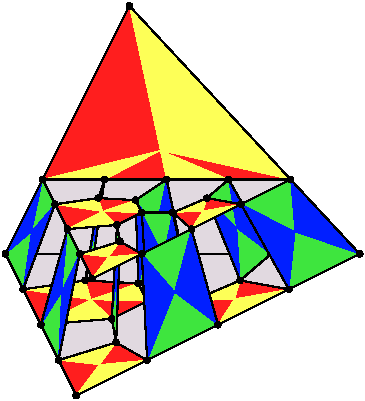
\includegraphics{pic-gcolor-ideal.pdf}
\end{center}
There are three of these arrangements,
each corresponding to the three ways of
partitioning the set of colors into two sets of two.
It follows that $\lie_{t_X,t_Z}$ 
is the direct sum of 6 disjoint ideals,
and specifically, that each Hamiltonian term in $H_{t_X,t_Z}$
lies in a single one of these ideals.
This result is crucial for obtaining the exact
diagonalization numerical results below.

%Colexes are discussed in \cite{Bombin2007exact}.
%The (bare) logical operators are derived in \cite{Bombin2015single} proposition 23.
%gauge fixing: \cite{Bombin2015}...
%error correction: \cite{Brown2015fault}
%equivelance to toric: \cite{Kubica2015unfolding}

%A complex lie algebra is the direct sum of simple ideals iff it is semisimple
%http://math.stackexchange.com/questions/405261/a-complex-lie-algebra-is-the-direct-sum-of-simple-ideals-iff-it-is-semisimple

%Representations of Direct Sum of Lie Algebras 
%http://math.stackexchange.com/questions/309617/representations-of-direct-sum-of-lie-algebras

%\todo{XXX How do ideals in the entire gauge group carry over into the semi-simple parts?}

\subsection{Lie algebra classification}

Here we explicitly compute decompositions of $\lie_{0,0}$
into the direct sum of simple Lie algebras.
First we review the classificiation of simple Lie algebras.

Let $n$ be the rank of a simple lie algebra $\mathfrak{g}.$
This is the dimension of the Cartan subalgebra $\mathfrak{h}.$
%This $n$ is also the subscript on the following Dynkin diagrams. 
%Dynkin used these to classify simple Lie algebras in 1947.
%The Cartan subalgebra $\mathfrak{h}$ is a maximal abelian Lie subalgebra 
%of $\mathfrak{g}.$

%Simple Lie algebras have connected Dynkin diagrams.
The simple Lie algebras are classified into four infinite series
$A_n, B_n, C_n, D_n$ as well as five other exceptional Lie
algebras that we will not need.

The $A_n$ series can be
constructed as 
$\mathfrak{sl}_{n+1}$ which are the traceless $(n+1)\times (n+1)$ matrices. 
Therefore the algebra dimension is $n^2 + 2n.$
%Number of roots is $n(n+1).$

For $n\ge 2$ the $B_n$ series 
comes from the Lie algebras
$\mathfrak{so}_{2n+1}$.
These can be constructed as $(2n+1)\times(2n+1)$ matrices
in block form 
$$
\left(\begin{array}{lll}
P & Q & T\\
R & S & U\\
V & W & 0\\
\end{array}\right)
$$
with $Q,R$ anti-symmetric and 
$P^{\top}=-S,T=-W^{\top},U=-V^{\top}.$
This algebra therefore has dimension $2n^2 + n.$
%Number of roots is $2n^2,$ number of short roots $2n.$

For $n\ge 3$ the $C_n$ series
comes from the Lie algebras
$\mathfrak{sp}_{2n}$.
These can be constructed as $2n\times2n$ matrices
in block form 
$$
\left(\begin{array}{ll}
P & Q \\
R & S
\end{array}\right)
$$
with 
$Q,R$ symmetric and $P^{\top}=-S.$
It follows that this algebra has dimension $2n^2 + n.$
%Number of roots is $2n^2,$ number of short roots $2n(n-1).$

For $n\ge 4$ the $D_n$ series
is $\mathfrak{so}_{2n}$.
These can be constructed as $2n\times2n$ matrices
in block form 
$$
\left(\begin{array}{ll}
P & Q \\
R & S
\end{array}\right)
$$
with $Q,R$ anti-symmetric and $P^{\top}=-S.$
Therefore this algebra has dimension $2n^2 - n.$
%Number of roots is $2n(n-1).$

%For $n\ge 1:$
%  \begin{tikzpicture}[scale=.4]
%    \draw (-1,0) node[anchor=east]  {$A_n$};
%    \foreach \x in {0,...,5}
%    \draw[xshift=\x cm,thick] (\x cm,0) circle (.3cm);
%    \draw[dotted,thick] (0.3 cm,0) -- +(1.4 cm,0);
%    \foreach \y in {1.15,...,4.15}
%    \draw[xshift=\y cm,thick] (\y cm,0) -- +(1.4 cm,0);
%  \end{tikzpicture}
%
%For $n\ge 2:$
%  \begin{tikzpicture}[scale=.4]
%    \draw (-1,0) node[anchor=east]  {$B_n$};
%    \foreach \x in {0,...,4}
%    \draw[xshift=\x cm,thick] (\x cm,0) circle (.3cm);
%    \draw[xshift=5 cm,thick,fill=black] (5 cm, 0) circle (.3 cm);
%    \draw[dotted,thick] (0.3 cm,0) -- +(1.4 cm,0);
%    \foreach \y in {1.15,...,3.15}
%    \draw[xshift=\y cm,thick] (\y cm,0) -- +(1.4 cm,0);
%    \draw[thick] (8.3 cm, .1 cm) -- +(1.4 cm,0);
%    \draw[thick] (8.3 cm, -.1 cm) -- +(1.4 cm,0);
%  \end{tikzpicture}
%
%For $n\ge 3:$
%  \begin{tikzpicture}[scale=.4]
%    \draw (-1,0) node[anchor=east]  {$C_n$};
%    \foreach \x in {0,...,4}
%    \draw[xshift=\x cm,thick,fill=black] (\x cm,0) circle (.3cm);
%    \draw[xshift=5 cm,thick] (5 cm, 0) circle (.3 cm);
%    \draw[dotted,thick] (0.3 cm,0) -- +(1.4 cm,0);
%    \foreach \y in {1.15,...,3.15}
%    \draw[xshift=\y cm,thick] (\y cm,0) -- +(1.4 cm,0);
%    \draw[thick] (8.3 cm, .1 cm) -- +(1.4 cm,0);
%    \draw[thick] (8.3 cm, -.1 cm) -- +(1.4 cm,0);
%  \end{tikzpicture}
%
%For $n\ge 4:$
%  \begin{tikzpicture}[scale=.4]
%    \draw (-1,0) node[anchor=east]  {$D_n$};
%    \foreach \x in {0,...,4}
%    \draw[xshift=\x cm,thick] (\x cm,0) circle (.3cm);
%    \draw[xshift=8 cm,thick] (30: 17 mm) circle (.3cm);
%    \draw[xshift=8 cm,thick] (-30: 17 mm) circle (.3cm);
%    \draw[dotted,thick] (0.3 cm,0) -- +(1.4 cm,0);
%    \foreach \y in {1.15,...,3.15}
%    \draw[xshift=\y cm,thick] (\y cm,0) -- +(1.4 cm,0);
%    \draw[xshift=8 cm,thick] (30: 3 mm) -- (30: 14 mm);
%    \draw[xshift=8 cm,thick] (-30: 3 mm) -- (-30: 14 mm);
%  \end{tikzpicture}

\subsection{A table of gauge code Lie algebras}

Using brute-force computation
we now find the dimension of the ideals in $\lie_{0,0}$
and therefore which simple Lie algebra these correspond to.
Note that here we switch back to
using $n$ to denote the number of qubits,
which in general is not the rank of the Lie algebra.
\begin{center}
\begin{tabular}{ l|c|c|c|l } 
model &\ $n$\ &\ $r$\ &\ $t_X$\ & $\mathfrak{g}_{t_X,0}$   \\
\hline
%    1D $XY$    &  7 &  6 & 0 & $D_7$   \\
%             &  8 &  6 & 0 & $D_4\oplus D_4$   \\
     1D $XY$  &  9 &  8 & 0 & $D_9$   \\
             & 10 &  8 & 0 & $D_5\oplus D_5$   \\
             & 11 &  10 & 0 & $D_{11}$   \\
             & 12 &  10 & 0 & $D_6\oplus D_6$   \\
\hline
    1D Ising & $4,...,16$  & $n-1$  & 0  & $D_n$   \\
\hline
    2D compass & 9 & 4 & 0 &  $A_{15}$  \\
            & 16 & 9 & 0 & $D_{256}$ \\
\hline
    3D gauge color & 15 & 6  & 0 & $6A_1$  \\
                & 39 & 18 & 0 & $6A_{7}$ \\
                & 65 & 32 & 0 & $4A_{31}\oplus 2A_{63} $  \\
\end{tabular}
\end{center}

This verifies the ideal decompositions we found in the
previous section, and also corroborates the large
amount of symmetry found with the orbigraph method.
For example, the $S_6$ symmetry of
the $n=15$ gauge color code corresponds to
%permutations of the six $\mathfrak{sl}_2$ ideals.
permutations of the six $A_1$ ideals.

There is a remaining mystery of where
the extra $\Z_2$ symmetry of the 2D compass model is coming from.
This symmetry was found with the orbigraph method in section~\ref{OrbigraphTable}.
It would be interesting if this symmetry turns out to be an element
of the Weyl group of the Lie algebra $\lie_{t_X,0}.$

%%%%%%%%%%%%%%%%%%%%%%%%%%%%%%%%%%%%%%%%%%%%%%%%%%%%%%%%%%%%%%%%%%%%%%%%%%%%%%%
%


%\section{Spectra}
%\label{spectra}

\section{Numerical results}

Here we show tables for the first and
second eigenvalues of the compass and gauge color code models.
These results are obtained using exact diagonalization methods.
For each instance we indicate the groundspace eigenvalue
$\lambda_1$ which is obtained from $H_{0,0}.$
Then we list the second eigenvalue of $H_{0,0}$ as
well as the first eigenvalue of $H_{t_X,0}$ for $t_X\ne 0.$
The weight of the corresponding frustrated stabilizer is $w(s_Z).$
%minimum number of gauge operators needed to form $s_Z.$
The eigenvalue closest to $\lambda_1(H_{0,0})$ is marked
with a tick, along with the value of the gap, $\lambda_1-\lambda_2.$
We only show the results for a single frustrated
stabilizer generator,
%\danbrowne{What is a frustrated stabiliser? You haven't explained what this is or how it is relevant.}
as it was confirmed numerically that 
%\danbrowne{Can you confirm something like this numerically? Or is a weaker statement true?}
adding further frustrated stabilizers never 
produces a better candidate for $\lambda_2.$
(This involved performing exact diagonalization on 
the top eigenvalues of every $H_{t_X,0}$ block in the Hamiltonian.)
Also, we only show non-isomorphic stabilizer generators,
under the lattice symmetry of the model.
We use the iterative solvers in software library 
{\tt SLEPc} \cite{Hernandez2005} to find these eigenvalues.

\begin{samepage}
\underline{2D compass code model}
\begin{center}
\begin{tabular}{ c|c|c|c|l|c } 
$n$ &  $t_X$    & $w(s_Z)$ & $\lambda_1$ & $\ \ \ \ \lambda_2$ ? & gap \\
\hline
\hline
16  &   0        &   &  19.012903&    16.335705          &            \\
&            & 8 &              &  18.369300    \checkmark & 0.643603 \\
\hline
25  &   0        &   & 29.076200 & 27.597280        &            \\
&            & 10 &              & 28.624004 \checkmark &  0.452196 \\
\hline
36  &   0        &   & 41.410454 & 40.585673        &            \\
&            & 12 &              & 41.094532 \checkmark &  0.315922 \\
%             &     &           &   &              &          &    &            \\
\end{tabular}
\end{center}
\end{samepage}

Such numerics for the 2D compass model have been previously found 
using similar methods \cite{Brzezicki2013}. 

\begin{samepage}
\underline{3D compass code model}
\begin{center}
\begin{tabular}{ c|c|c|c|l|c } 
$n$ &  $t_X$    & $w(s_Z)$ & $\lambda_1$ & $\ \ \ \ \lambda_2$ ? & gap \\
\hline
\hline
27  &   0        &   & 60.295471  &    58.382445          &            \\
&            & 18 &              &  59.757677   \checkmark & 0.53779 \\
\end{tabular}
\end{center}
\end{samepage}

\begin{samepage}
\underline{3D gauge code model}
\begin{center}
\begin{tabular}{ c|c|c|c|l|c } 
$n$ &  $t_X$    & $w(s_Z)$ & $\lambda_1$ & $\ \ \ \ \lambda_2$ ?  & gap \\
\hline
\hline
15  & 0         & &  25.455844  & 16.970563    &  \\
                 &   & 8 &              & 22.214755 \checkmark & 3.241089           \\
\hline
%39  & 0         & &  64.476081   & 58.137233    &  \\
%                 &           & 8 &              & 60.706477    &   \\
%                 &           & 8 &              & 60.357053  &    \\
%                 &           & 12 &              & 61.366348   &  \\
%                 &           & 20 &              & 63.495916  \checkmark  & 0.980165 \\
%\hline
65  & 0         &    &  104.076026  & 99.014097     &    \\
                 &           & 8  &              &  100.429340   &            \\
                 &           & 12 &              &  100.585413   &            \\
                 &           & 12 &              &  101.602340   &            \\
                 &           & 18 &              &  102.382483  \checkmark  &  1.693543 \\
\hline
175 & 0         &  &  267.197576  & 264.250644    & \\
 & & 8  & & 263.171190  &    \\
 & & 8  & & 263.324858  &    \\
 & & 8  & & 263.340832  &    \\
 & & 12 & &  264.269635  &    \\
 & & 12 & &  264.617135  &    \\
 & & 12 & &  264.745548  &    \\
 & & 18 & &  264.843629  &    \\
 & & 18 & &  265.413935  &    \\
 & & 18 & &  265.754772  &    \\
 & & 24 & &  266.148188  \checkmark &  1.04939  \\
\end{tabular}
\end{center}
\end{samepage}

\begin{figure*}
\begin{center}
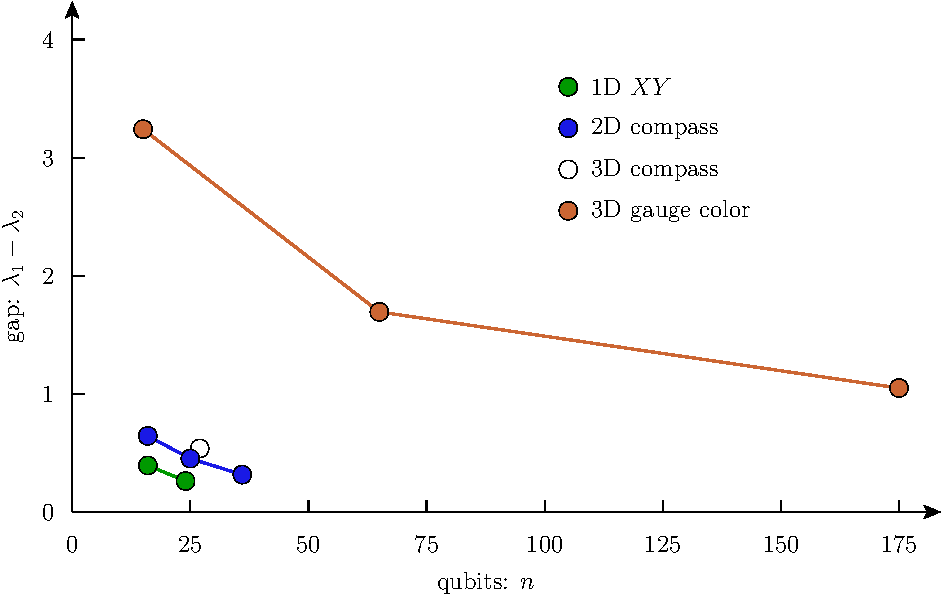
\includegraphics[width=1.0\columnwidth]{pic-gap.pdf}
\caption{The spectral gap of four different gauge code Hamiltonians, versus the number
of qubits $n$. The gap is defined as the difference between
the ground eigenvalue and the first excited eigenvalue.
These results are obtained by exact diagonalization.
}
\label{PicGap}
\end{center}
\end{figure*}

\begin{figure*}
\begin{center}
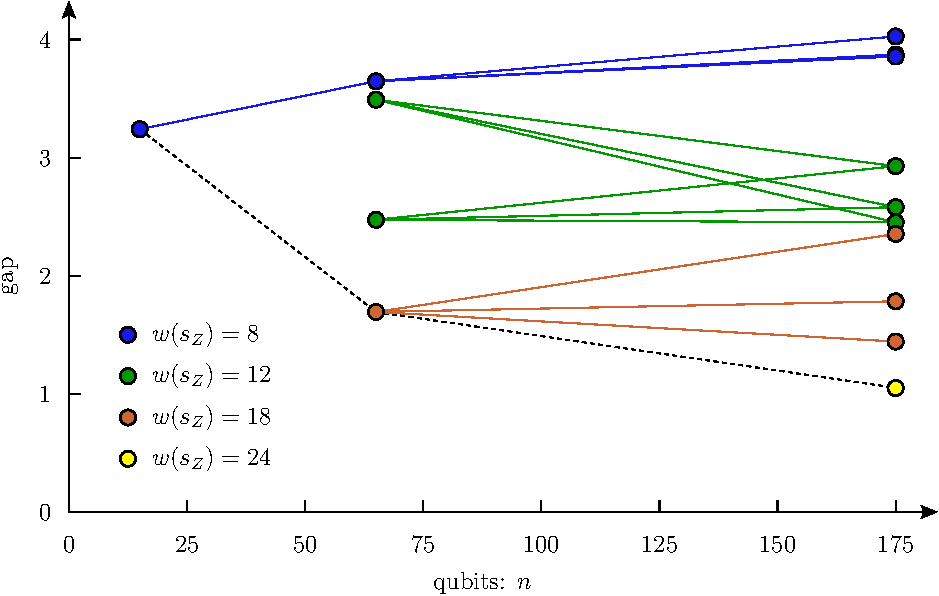
\includegraphics[width=1.0\columnwidth]{pic-gap-stabs.pdf}
\caption{
Here we show the spectral gap
for each Hamiltonian block $H_{t_X,0}$
of the 3D gauge color code models of sizes $n=15,$ $n=65$ and $n=175.$
This gap is defined as $\lambda_1(H) - \lambda_1(H_{t_X,0}).$
Each point is colored according to the weight of the
frustrated stabilizer generator.
}
\label{PicGapStabs}
\end{center}
\end{figure*}

The gap of the 3D gauge color code is clearly far more
robust than the other models, see Figure \ref{PicGap}.
%This is solely due to the geometry of the code...
It does decrease with $n$, but note also that the
stabilizers in the code are also growing, up to weight 24.
To emphasize this point we show in Figure \ref{PicGapStabs}
the ground eigenvalues of all of these blocks $H_{t_X,0}.$
For larger codes in this family the stabilizers do not get
bigger than weight 24.
%They do not get any bigger after this.
It is not clear to what extent these results are
representative of larger code sizes, but we
can already see from Figure \ref{PicGapStabs} 
evidence that 
the weight of the frustrated stabilizer generator plays a more
important role than the size of the code itself.

%\danbrowne{Does this mean that small codes are not representative of generic codes?}

There are two main points to make about these numerics.
The first is that the gap of the compass model 
is decreasing much faster than the gap in the gauge color model.
In fact, there is strong evidence \cite{Dorier2005} 
that the gap of the compass model
tends to zero as the lattice size grows.
The second point to make
is that the gap always corresponds to frustrating
a stabilizer ($t_X\ne 0.$) 
Moreover, the stabilizer that
gives rise to the gap is the one with largest weight.
This is a crucial connection to make because the
stabilizers of the compass model grow with the linear
size of the model
while those of the gauge color model
do not need to grow beyond a constant bound.
%Note the similar
%behaviour of the 1D $XY$-model and transverse field Ising model.
This would suggest that if this is the mechanism for
gapless behaviour that the gauge color model may
be gapped.

The above numerics reach the limit of presently available 
computational resources.
To find eigenvalues for each Hamiltonian block $H_{t_X,0}$
%and for the compass code and gauge color codes we found ...)
%For simulation purposes, these numerics are constrained by
we need to operate on wavefunctions with $2^r$ real coefficients.
The iterative solvers in {\tt SLEPc} need to store at least two,
but ideally more, of these wavefunctions.
For $r=32$ this is about 32 Gigabytes for one wavefunction (using double
precision coefficients) and so this value for $r$ is roughly the
upper limit on these numerical techniques.
Without decomposing the gauge color code into six disjoint ideals
it would be impossible to obtain the results for the $n=175$ code,
as this code has $r=94$.
%\danbrowne{Very nice results. Why did you stop at n=175? What computational resources were required to achieve that?}

\section{Cheeger cuts}

In this final section of Chapter 2 
we give some heuristic
arguments for why the size of the stabilizers is
related to the gap of the code. 
%This does not lead to 
%definitive conclusions. It appears that much more 
%work is required.

The Perron-Frobenius structure theory places
strong constraints on the first and second
eigenvectors of $\Gamma_{t_X}:$
the first eigenvector has all positive entries,
%and the second eigenvector does not.
and therefore all vectors orthogonal to the first
eigenvector will have both positive and negative entries.
In general, the set of edges of $\Gamma_{t_X}$ where
such a vector changes sign we call a Cheeger cut 
\cite{Cheeger1970,Chung1997}.
(We ignore the possibility that this vector
may have zero entries.)
The Cheeger cut associated to the second eigenvector
is particularly important, and we next show an
example of how this cut relates to the gap.

\subsection{The double well model is gapless}

We consider a linear graph Hamiltonian
with a ``double-well'' potential.
This does not correspond to any gauge code Hamiltonian.
The state space will be $d$ dimensional with
basis vectors numbered $\ket{1},...,\ket{d}.$
We take
$ \Ham = A + U $
with
$$
A_{ij} = \left\{ \begin{array}{ll}
     1 &\mbox{if}\  |i-j|=1,  \\
     0 &\mbox{otherwise}\end{array}\right.
\ \ \mbox{and}\ \ 
U_{ij} =  \left\{ \begin{array}{ll}
     2 &\mbox{if}\  i=j=1 \ \ \mbox{or}\ \  i=j=n, \\
     0 &\mbox{otherwise.}\end{array}\right.
$$
$A$ here is a kind of transition matrix,
and $U$ is a diagonal potential energy term.

For $d\gg 1$, the largest
eigenvalue is $\lambda_1 \cong \frac{5}{2}$.
The corresponding eigenvector $\ket{v_1}$
has all positive components that
decay exponentially away from the well sites
at $\ket{1}$ and $\ket{d}:$
$$
    \braket{i}{v_1} 
    \cong 2^{i-1} \braket{1}{v_1}
    \ \ \mbox{for}\ \ i\ll \frac{d}{2}.
$$
For the second eigenvalue, $\lambda_2$
we also have  $\lambda_2 \cong \frac{5}{2}$
and indeed, as $d$ grows
the gap $\lambda_1 - \lambda_2 \rightarrow 0$
and so this model is gapless.

Here we depict the wavefunctions for
the first two eigenvectors for a system with $d=12:$
\begin{center}
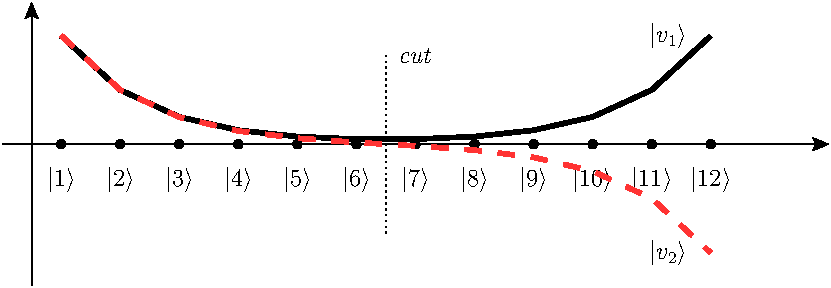
\includegraphics[]{pic-dwell.pdf}
\end{center}
The simplest way to show this model
is gapless is using a variational
argument.
Any another vector $\ket{u}$
that is orthogonal to the groundspace
vector will have $\bra{u}H\ket{u} \le \lambda_2.$
To construct a candidate for $\ket{u}$
partition the
basis vectors into two parts:
$$
    \Gamma = \Gamma_A \cup \Gamma_B
$$
and write $\ket{v_1} = 
\ket{v_A}\oplus\ket{v_B}$
as well as Hamiltonian with this
decomposition as
$$
H = 
\left(\begin{array}{ll}
H_{AA} & H_{AB} \\
H_{BA} & H_{BB}
\end{array}\right).
$$
Now let
$$
    \ket{u} = \ket{v_A} \oplus -\ket{v_B}
$$
%$$
%\braket{i}{u} =
%    \left\{ \begin{array}{ll}
%     +\braket{i}{v_1} &\mbox{if}\ \ket{i}\in\Gamma_A \\
%     -\braket{i}{v_1} &\mbox{if}\ \ket{i}\in\Gamma_B\end{array}\right..
%$$
And then
\begin{align*}
    \lambda_2 \ge \bra{u}H\ket{u} &= 
\bra{v_A}H_{AA}\ket{v_A} +
\bra{v_B}H_{BB}\ket{v_B} -
\bra{v_B}H_{BA}\ket{v_A} -
\bra{v_A}H_{AB}\ket{v_B} \\
    &= \lambda_1 - 4 \bra{v_B}H_{BA}\ket{v_A}.
\end{align*}
So if we can show that 
$ \bra{v_B}H_{BA}\ket{v_A}$
tends to zero we are done.
This term involves the 
dynamical coupling between the
groundstate wavefunction along
the cut between $A$ and $B$.
To succeed we must find such a cut where
the wavefunction is small. In general
this appears to be quite difficult,
even though in the models we are considering
numerics show that not only is the
wavefunction small away from potential wells
but it is exponentially small.

%In summary, we note the important
%features of this model.
%The groundstate wavefunction has all
%positive components, which implies
%that the size of the gap is controlled
%by the ``weight'' of a cut.
%Also, we are hinting at the role
%of symmetry as these cuts will
%turn out to be reflection lines
%under certain symmetries of the models
%we consider.


\subsection{The cut and symmetry}

We now study 
the cut associated to the second eigenvector of a 
weakly self-dual gauge Hamiltonian $H,$
and relate this to the stabilizers of the code.
The key realization is that $\Gamma_{t_X}$ is like
the double well potential above,
but now we have $2^{m_X}$ such wells,
that is, one for every $s_X\in \Span{S_X}.$
This is clear from examining the basis vectors for $\Gamma_{t_X}.$
These are 
$$
    \ket{v S_X + u R_X + t_X}, \smbox{where} v\in \Field_{m_X}, u\in\Frd
$$
and those that satisfy the most $G_Z$ terms are
precisely those with $u=0.$

We already know this is either the second eigenvector of $H_{0,0}$
or otherwise the first eigenvector of $H_{t_X,0}$ for some $t_X \ne 0.$
To relate this to the Perron-Frobenius theory we note the 
decomposition:
$$
    \Gamma_{t_X} = \bigoplus_{t_Z\in\Span{T_Z}} H_{t_X, t_Z}.
$$
This gives the spectral decomposition of each graph $\Gamma_{t_X}$ 
in terms of ``momenta'' $t_Z.$

We focus on $\Gamma_0.$
This must contain the second eigenvector of $H$ by weak self-duality of the code.
%The matrices $H_{0,t_Z)}$ are Perron-Frobenius (by a change of basis)
%and so the first eigenvector $v_1(H_{0,t_Z})$ can be taken to be positive.
$X$ type stabilizers $s_X\in S_X$ act on the $0,t_Z$ irreps in $\Gamma_0$
by $\pm 1$ according to the commutator $[[s_X, t_Z]].$
Suppose the second eigenvector of $H$ lives in
$H_{0,t_Z}$ for $t_Z\ne 0$. 
Let $s_X\in S_X$ with $[[s_X, t_Z]]=-1.$
Then we must have an odd number of Cheeger cuts 
on every $\Gamma_0$ path between $\ket{v}$ and $s_X\ket{v}$ for all basis
vectors $\ket{v},$ that is, $v\in\Span{S_X}\oplus\Span{R_X}.$

In a similar vein, if the second eigenvector of $H$ lives in $H_{0,0}$
then we must have an even number of Cheeger cuts 
on every $\Gamma_0$ path between $\ket{v}$ and $s_X\ket{v}$ for all stabilizers $s_X\in S_X$
and basis vectors $\ket{v}.$

In summary, the idea is that large stabilizers lead to
widely separated well potentials and hence gapless behaviour,
while stabilizers of bounded weight force the cuts to
appear close to the wells and hence maintain a gap.
Even though numerics show the wavefunction becoming 
exponentially small away from well potentials,
it is also exponentially wide.
So making these arguments rigorous appears to be difficult.

The following fact would appear to be true under certain conditions,
but is not at all true for example when $T$ is trivial:
\begin{framed}
\noindent{\bf Proto-fact:}
For a sufficiently ``well-behaved''
weakly self-dual
gauge code Hamiltonian $H$
\begin{align*}
\lambda_2(\Ham) 
    &= \min_{t_X\ne 0} \lambda_1(\Ham_{t_X,0})\\
    &= \min_{t_Z\ne 0} \lambda_1(\Ham_{0,t_Z}).
\end{align*}
\end{framed}
Indeed, contrary to this proto-fact
we suspect that $H_{0,0}$ will not be gapped in
the generic case. 
Numerics suggest that
there is no lower bound on the gap of 
randomly constructed stabilizer-less gauge code Hamiltonians.
Perhaps double well behaviour can still be imitated even without
stabilizers: merely having a large region of almost-stabilizer
behaviour (large shallow well) could be enough to send the gap to zero.

There are also results that state that generic 
local Hamiltonians are gapless \cite{Movassagh2016}.

\subsection{Cheeger inequalities}

We saw above how the Cheeger cut gives a variational ansatz
for building a second eigenvector to the Hamiltonian and hence
an upper bound on the gap.

In this section we show how the Cheeger cut also 
yields a lower bound on the gap.
%an upper bound on the second eigenvalue of a Perron-Frobenius
%operator $H.$

In \cite{Friedland2002}, they derive the following Cheeger inequality
by considering bi-partitions of the graph. We will do the
same, but using matrix block notation.

Let $v_2$ be a second eigenvector, $ \Ham v_2 = \lambda_2 v_2 $ 
and $||v_2||=1$.
We bi-partition the space 
so that $v_2$ has (vector) blocks:
$$
v_2 = \left( \begin{array}{l}
x\\
y\end{array} \right)\quad
$$
with $x\ge 0$ and $y\le 0,$ component-wise.
Let the blocks of $\Ham$ under the same partition be:
$$
\Ham = \left( \begin{array}{ll}
A&C\\
C^\top&B\end{array} \right).\quad
$$
If we denote $\lambda_1(A)$ as the top eigenvalue of $A$ and
$\lambda_1(B)$ as the top eigenvalue of $B$,
then
\begin{align*}
\lambda_2 = v_2^\top \Ham v_2 &= x^\top A x + 2 x^\top C y + y^\top B y \\
        &\le x^\top A x + y^\top B y\ \le\ ||x||^2 \lambda_1(A) + ||y||^2 \lambda_1(B) \\
        &\le \mbox{min}(\lambda_1(A), \lambda_1(B))\ \le\ \lambda_1.
\end{align*}

Defining the following constant as a maximization over
all bi-partitions of $\Ham:$
$$
    \nu(\Ham) := \max_{A, B}\ \mbox{min}(\lambda_1(A), \lambda_1(B))
$$
the above calculation shows that
$$
    \lambda_2 \le \nu(\Ham) \le \lambda_1.
$$

%To bound $\lambda_2$ from below, we use a variational argument.
%For any unit vector $v$ orthogonal to the top eigenspace of $\Ham$ we
%have $v^\top \Ham v \le \lambda_2.$

\section{Summary}

\danbrowne{Needs a concluding section summarising results and discussing open questions and potential research directions. }

In section 1 we apply general principles of group
representation theory to block diagonalize Hamiltonians.
The terms of the Hamiltonian generate a group (by multiplication),
and we also have a ....
\todo{fixme}

In summary, we have the complete representation
theory for $CSS$ gauge code Hamiltonians.

analyse spectrum of weakly self-dual $CSS$ gauge code
Hamiltonians using Perron-Frobenius theory.

It is clear from numerics that nothing as simple as the proto-fact
holds. Roughly speaking, larger stabilizers lead to gapless behaviour,
but 

more models need to be considered,  numerics obtained,
including codes chosen from random ensembles.

The Cheeger inequalities are a first attempt to
relate the gap to the geometric structure of the
graph $\Gamma$, in particular the size of stabilizers.
This analysis is too weak to show any result, and so
further work is needed.
If this approach is to succeed, a much sharper
bound on the shape of the wavefunction is needed.

The perturbation theory for stabilizer Hamiltonians has good
results, we would also want something like this for gapped
gauge code Hamiltonians, to establish physicality.

We leave as an open problem 
to extend the representation theory of
CSS gauge codes in section 2.4 to arbitrary gauge codes
(not necessarily satisfying the CSS condition).
We do not need this in the present work.


%%%%%%%%%%%%%%%%%%%%%%%%%%%%%%%%%%%%%%%%%%%%%%%%%%%%%%%%%%%%%%%%%%%%%%%%%%%%%%%
%

%\subsection{The compass model is gapless}
%
%Although there is strong evidence that the gap dissapears as the lattice size
%$l$ grows, it is still worthwhile considering the exact reasons for this.
%
%We use a variational argument to show that $\lambda_1(H_{t_X,0})$
%is close to $\lambda_1(H_{0,0}).$
%Given the similarity of the form of these two blocks, we
%take the ground eigenvector $v_1$ of $H_{0,0}$ and apply it
%to $H_{t_X,0}$. % where $t_X$ has low weight.
%Recall that we identified the bases of these two Hamiltonian blocks.
%\begin{align*}
%    \lambda_1 - \lambda_2 &\le \bra{v_1}H_{0,0}\ket{v_1} - \bra{v_1}H_{t_X,0}\ket{v_1}  \\
%            &= \bra{v_1}(H_{0,0} - H_{t_X,0})\ket{v_1}  \\
%    &= \sum_{v\in\Frd} 2\bigl(w(G_Z R_X^\top v^\top + G_Z t_X^\top) -w(G_Z R_X^\top v^\top)\bigr) 
%    |\braket{v}{v_1}|^2.
%\end{align*}
%
%FAIL

%%%%%%%%%%%%%%%%%%%%%%%%%%%%%%%%%%%%%%%%%%%%%%%%%%%%%%%%%%%%%%%%%%%%%%%%%%%%%%%
%

%\subsection{Perturbation of the Perron vector}
%
%Here we note the relation of
%perturbations to the Perron-Frobenius theory.
%
%Let $A$ be non-negative irreducible $n\times n$ matrix.
%Let $v\ne 0$ be a non-negative $n$ vector, and $B = A + \ket{e_i}\bra{v}.$
%Then 
%$$
%\frac{y_i}{x_i} > \frac{y_j}{x_j} \ \ \mbox{for}\ \ j \ne i,
%$$
%where $x, y$ are the Perron eigenvectors of $A, B$ respectively
%\cite{Elsner1982}.
%
%Let $H(t)$ be non-negative irreducible matrix, continuously
%differentiable wrt $t.$
%Let $v(t)$ and $\lambda(t)$ be the Perron eigenvector and value of $H(t)$
%with $\braket{v}{v}=1.$
%Then
%$$
%    \lambda' = \bra{v}H'\ket{v}
%$$
%and
%$$
%    \ket{v'} = -(H-\lambda)^{-1}(H' - \lambda')\ket{v}.
%$$
%where $(H-\lambda)^{-1}$ is the Moore-Penrose inverse of $H-\lambda.$ See \cite{Meyer1988}.


%%%%%%%%%%%%%%%%%%%%%%%%%%%%%%%%%%%%%%%%%%%%%%%%%%%%%%%%%%%%%%%%%%%%%%%%%%%%%%%
%
%%%%%%%%%%%%%%%%%%%%%%%%%%%%%%%%%%%%%%%%%%%%%%%%%%%%%%%%%%%%%%%%%%%%%%%%%%%%%%%
%


%\subsection{Discussion}
%
%In \cite{AlShimary2010}, they 
%build a kind of graph laplacian from a known ground state:
%``This is not a major drawback as there
%are large families of physically relevant states, e.g. the
%Matrix Product States, that are ground states of Hamil-
%tonians which are not known to be gapped or not in two
%or higher dimensions. Such an important example is
%the two-dimensional AKLT model that can support uni-
%versal quantum computation by measurements only, but
%it is not proven yet if it is gapped which would establish
%its fault-tolerance.''
%This Laplacian has the same gap as the Hamiltonian.
%
%It would be nice to connect geometric properties of the
%graph to spectral gap properties. For example, the spectral gap of
%the normalized graph laplacian can be bounded from below
%by the Coarse Ricci curvature \cite{Lin2011}. 
%Unfortunately, it appears
%that there are no good connections between the spectrum
%of the normalized graph laplacian and the spectrum of the adjacency matrix.
%% http://mathoverflow.net/questions/118870/connection-between-eigenvalues-of-matrix-and-its-laplacian
%
%See also \cite{Jarret2014,Jarret2015}. 
%In \cite{Jarret2015modulus} they
%write the Hamiltonian as a sum of the
%the combinatorial graph Laplacian and a (diagonal) potential, 
%and then employ methods from PDE theory \cite{Andrews2011}.
%Also: \cite{Baume2016}. % Michaels' Phd thesis
%
%We expect generic local Hamiltonians to be gapless \cite{Movassagh2016}.

%Suzuki-Trotter expansions
%https://en.wikipedia.org/wiki/Baker%E2%80%93Campbell%E2%80%93Hausdorff_formula

%%%%%%%%%%%%%%%%%%%%%%%%%%%%%%%%%%%%%%%%%%%%%%%%%%%%%%%%%%%%%%%%%%%%%%%%%%%%%%%
%
%%%%%%%%%%%%%%%%%%%%%%%%%%%%%%%%%%%%%%%%%%%%%%%%%%%%%%%%%%%%%%%%%%%%%%%%%%%%%%%
%

%\section{Outlook}
%
%There's a growing zoo of these systems and little is known
%about their energetics, in particular if they are gapped or
%not as the size increases.
%
%A family of topological subsystem codes,
%from the code perspective  \cite{Bombin2010,Bombin2014,Suchara2011},
%from the cond-mat (integrals of motion!) perspective:
%\cite{Kargarian2010,Bombin2009}
%Topological subsystem Codes: \cite{Suchara2011}
%Structure of 2D Topological Stabilizer Codes: \cite{Bombin2014}
%Gauge color codes, gauge fixing: \cite{Bombin2015}
%Gauge color codes, single shot: \cite{Bombin2015single}
%
%A generalization of this is the 
%monomial formalism \cite{Van2011}. 
%These operators also form a group and would
%have a corresponding representation theory.


%% CUT HERE
%\appendix
%% CUT HERE

%\label{appendix}

